\documentclass[aspectratio=169]{beamer} % Formato widescreen per il diagramma a blocchi

% --- IMPOSTAZIONI TEMA ---
\usetheme{Madrid}
\usecolortheme{whale}
\setbeamertemplate{navigation symbols}{} % Rimuove i simboli di navigazione in basso
\setbeamertemplate{caption}[numbered]

% --- PACCHETTI STANDARD ---
\usepackage[utf8]{inputenc}
\usepackage[T1]{fontenc}
\usepackage[italian]{babel}
\usepackage{lmodern} % RISOLVE IL WARNING SUI FONT BOLD
\usepackage{amsmath, amsfonts, amssymb}
\usepackage{booktabs} % Per tabelle più belle
\usepackage{caption}
\usepackage{subcaption}
\usepackage{bm}
\usepackage{siunitx}
\usepackage{colortbl}
\usepackage{pifont}
% --- PACCHETTI PER GRAFICA E SCHEMI (TIKZ) ---
\usepackage{tikz}
\usetikzlibrary{shapes.geometric, arrows.meta, fit, calc, positioning, backgrounds}


\usepackage{graphicx}
\graphicspath{{../../img/}{../../img/controllo_verticale/}}
\renewcommand{\figurename}{Fig.}

% --- METADATI ---
\title{Modellazione dinamica e design del controllo per un innovativo VTOL}
\author{}
\date{}

\begin{document}

% --- SLIDE TITOLO ---
\begin{frame}
    \titlepage
    \begin{center}
        Università degli Studi di Roma Tor Vergata\\
    Dipartimento di Ingegneria
    \end{center}
    
\end{frame}

% --- INDICE ---
\begin{frame}{Sommario}
    \tableofcontents
\end{frame}

% ============================================================
% PARTE 0: INTRODUZIONE
% ============================================================
\section{Introduzione}

\begin{frame}
    \vfill
    \centering
    {\Huge \textbf{Introduzione}}
    \vfill
\end{frame}

\begin{frame}{Introduzione}
    L'interesse per gli UAV è in forte crescita (sorveglianza, agricoltura, search and rescue).
    Tuttavia, le configurazioni classiche presentano limitazioni:

    \vspace{0.2cm}
   \begin{columns}[t]
        \column{0.48\textwidth}
        \textbf{Multirotori}
        \begin{itemize}
            % NOTA: Le parentesi graffe { } extra servono a proteggere il comando nel beamer
            \item[{\textcolor{green}{\checkmark}}] Semplicità, Hovering stabile.
            \item[{\textcolor{red}{$\times$}}] Bassa efficienza, Range ridotto.
        \end{itemize}
        \centering
        \begin{figure}
            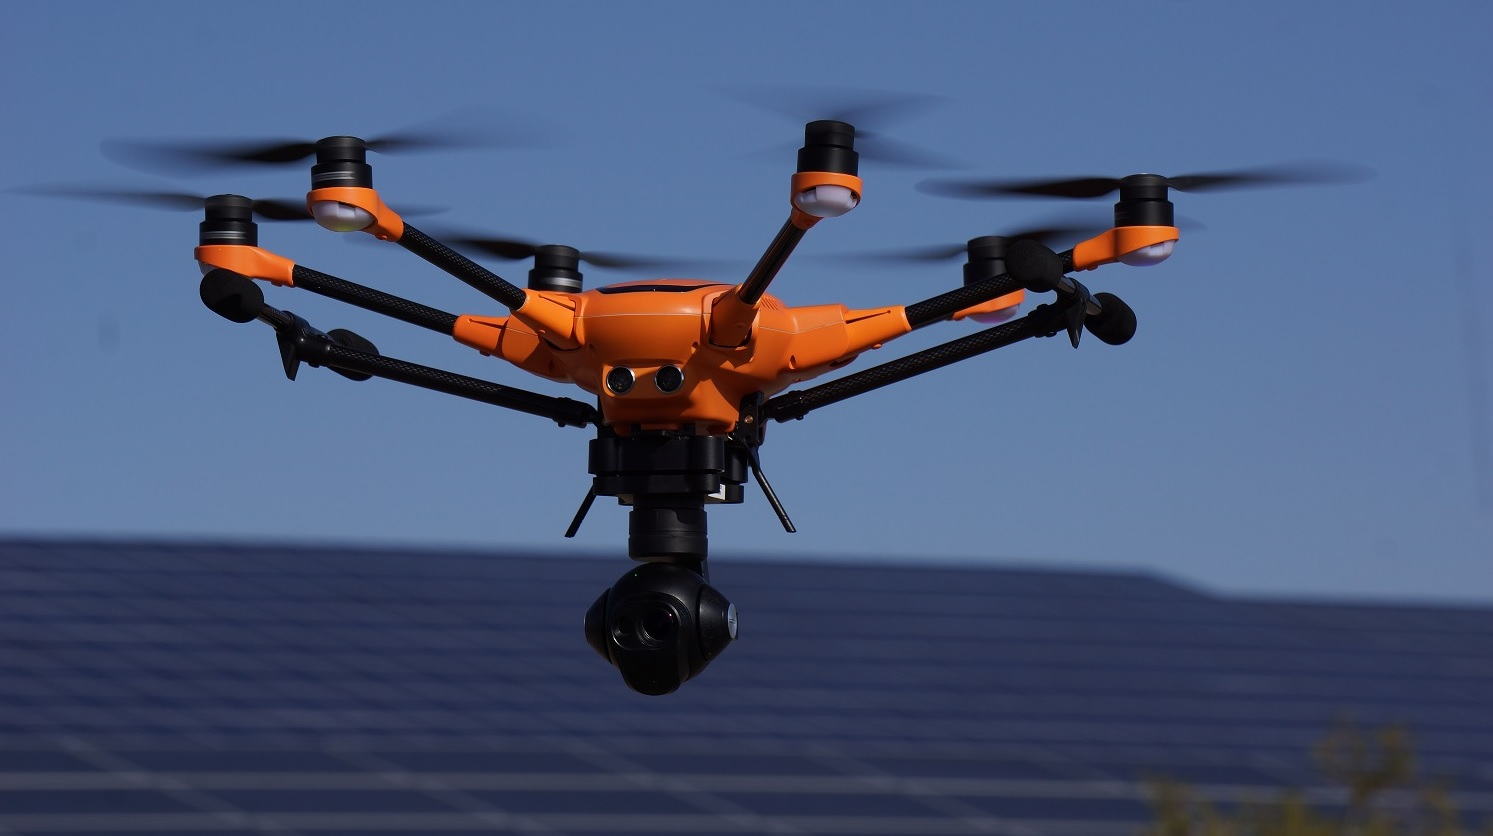
\includegraphics[width=0.6\textwidth]{multicopter.png}
            \caption{multicottero}
        \end{figure} 
        
        \column{0.48\textwidth}
        \textbf{Ala Fissa}
        \begin{itemize}
            \item[{\textcolor{green}{\checkmark}}] Alta efficienza, Lungo raggio.
            \item[{\textcolor{red}{$\times$}}] Necessità piste, No hovering.
        \end{itemize}
        \centering
        \begin{figure}
            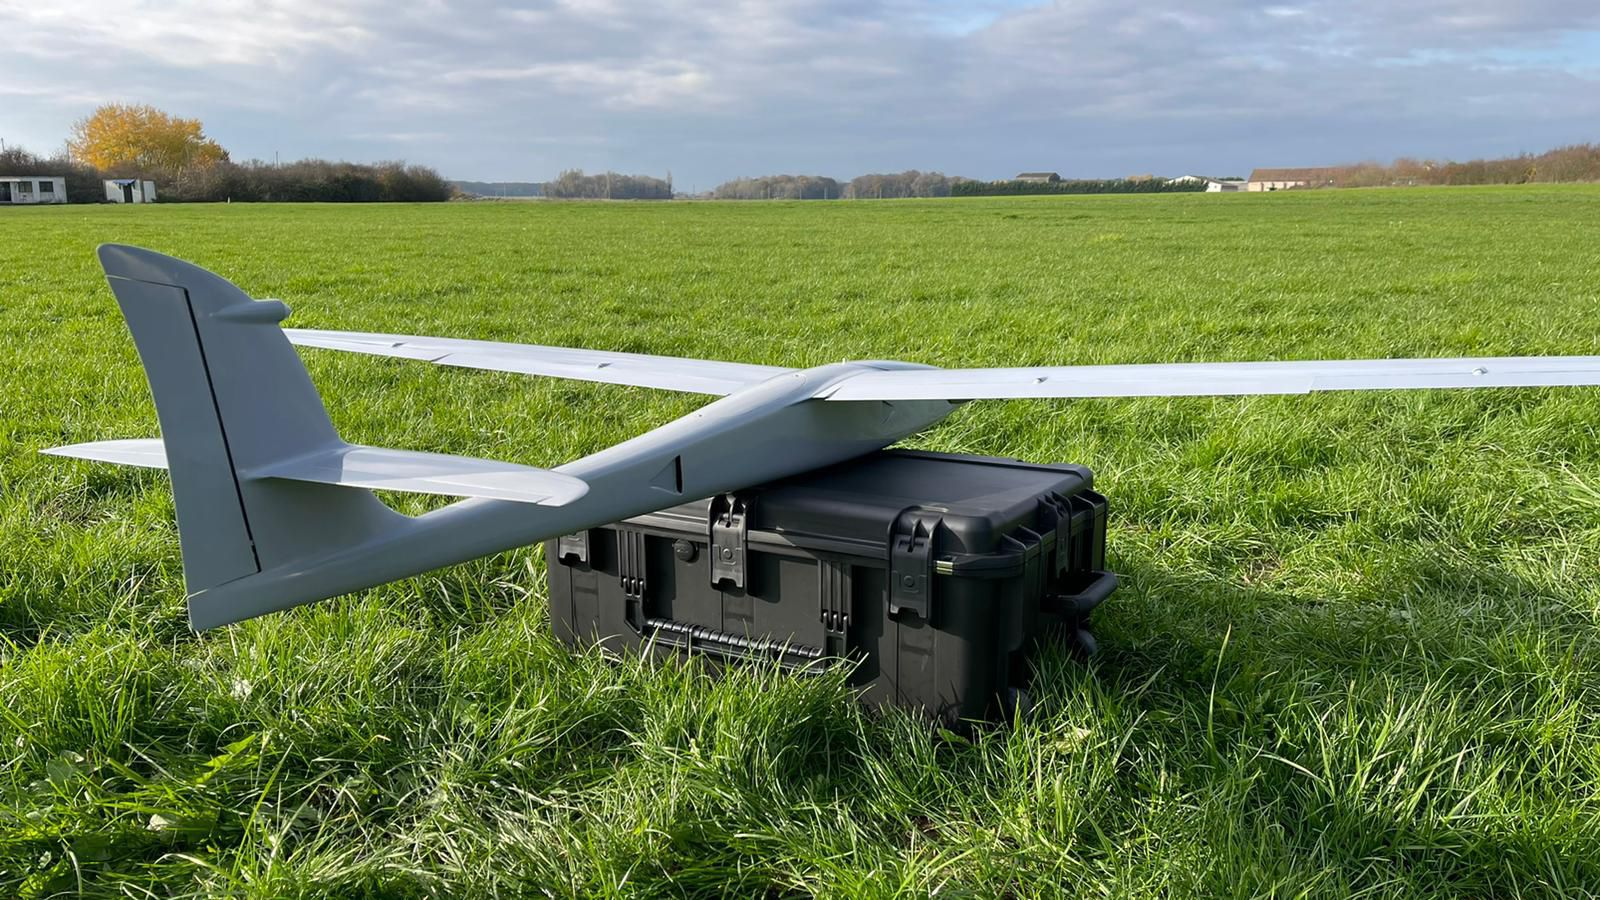
\includegraphics[width=0.6\textwidth]{fixed_wing.png}
            \caption{aereo}
        \end{figure}       
    \end{columns}

    % \vspace{0.2cm}
    \centering
    \textbf{Soluzione:} Configurazione Ibrida (VTOL)
\end{frame}

\section{Descrizione VTOL}

\begin{frame}
    \vfill
    \centering
    {\Huge \textbf{Descrizione VTOL}}
    \vfill
\end{frame}

\begin{frame}{VTOL tilting-rotor}
    Il tricottero \textit{tilting-rotor} combina i benefici delle due architetture:
    
    \begin{columns}
        \column{0.6\textwidth}
        \begin{itemize}
            \item \textbf{Decollo/Atterraggio:} Verticale (come un elicottero), indipendente da infrastrutture.
            \item \textbf{Crociera:} Volo aerodinamico (come un aereo) ruotando i propulsori.
        \end{itemize}
        
        \vspace{0.5cm}
        \begin{block}{La Sfida Ingegneristica}
            Questa versatilità introduce una \textbf{dinamica complessa} e fortemente accoppiata, 
            richiedendo strategie di controllo e allocazione avanzate.
        \end{block}

        \column{0.4\textwidth}
        \centering
        \begin{figure}
            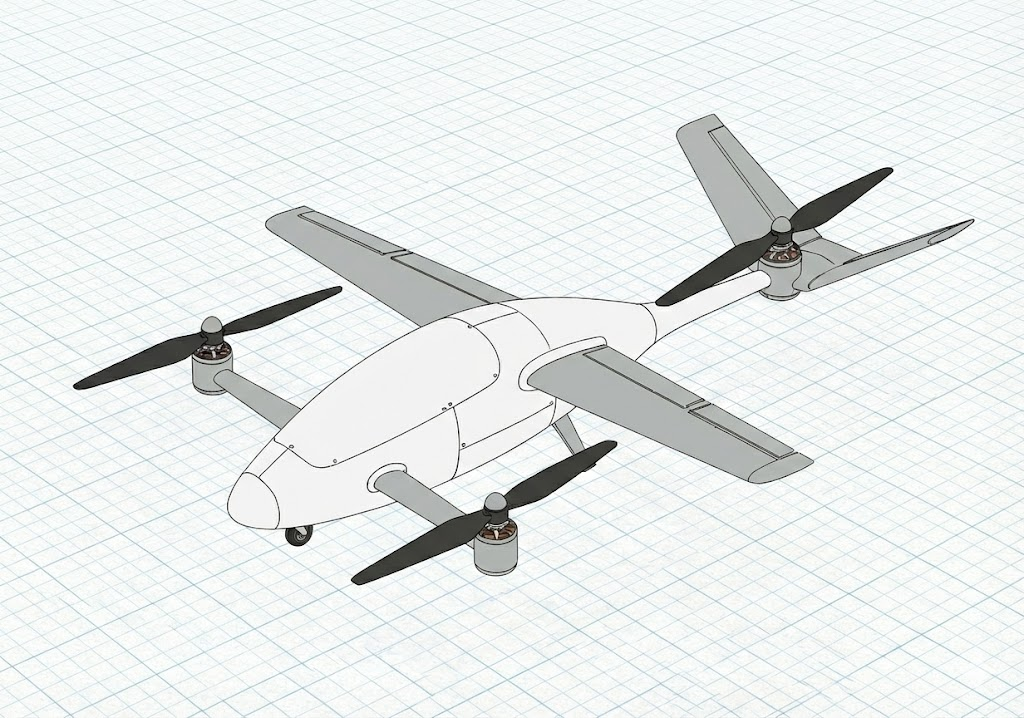
\includegraphics[width=0.8\textwidth]{VTOL.png}
            \caption{\footnotesize Rendering del velivolo.}
        \end{figure}
        
    \end{columns}
\end{frame}

\begin{frame}{Tricottero tilting-rotor}
    \begin{columns}[c] % [c] centra verticalmente il contenuto delle colonne
        \column{0.55\textwidth}
        Nello specifico, il tricottero in esame presenta i rotori orientabili, ma non ha superfici geometriche variabili.
        
        \vspace{0.5cm} % Un po' di respiro tra i paragrafi
        Questa configurazione rappresenta una criticità in fase di crociera perché è necessario gestire sia assetto che posizione solo tramite la vettorizzazione della spinta.

        \column{0.45\textwidth}
        \begin{figure}
            \centering
            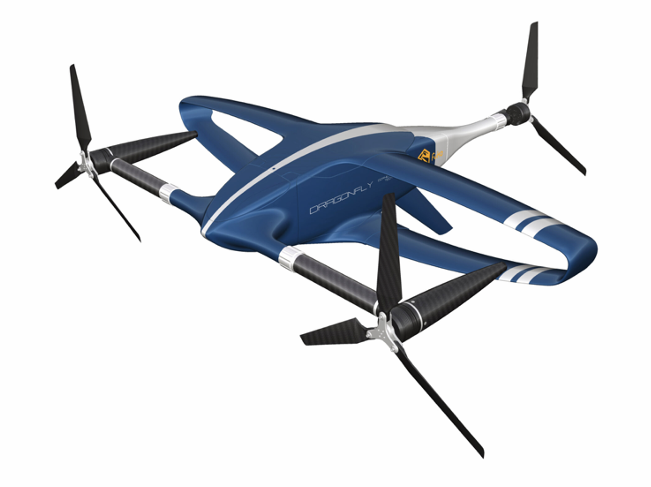
\includegraphics[width=\columnwidth]{dragonfly.png} 
            \caption{Dragonfly.}
        \end{figure}
    \end{columns}
\end{frame}

% ============================================================
% 2. MODELLAZIONE (RIELABORATA)
% ============================================================
\section{Modello Matematico}

\begin{frame}
    \vfill
    \centering
    {\Huge \textbf{Modello Matematico}}
    \vfill
\end{frame}

% --- SLIDE 1: SISTEMI DI RIFERIMENTO ---
% Mantenuta simile, pulita la formattazione
\begin{frame}{Sistemi di Riferimento}
    \small
    Per descrivere la dinamica 6-DOF si adottano due sistemi destrorsi:
    \vspace{-0.5cm}
    \begin{columns}[t]
        \begin{column}{0.5\textwidth}
            \begin{itemize}
                \item \textbf{Inerziale ($\mathcal{F}_g$):} \\
                Posizione $\bm{P}_g$, Assetto $\bm{\Theta}_g$ (Eulero).
                \begin{center}
                    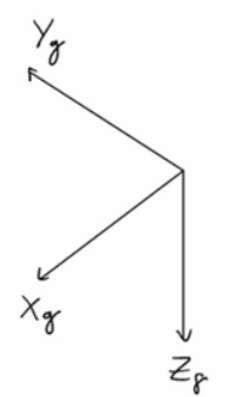
\includegraphics[height=3cm]{sist_rif_global.png}
                    \captionof{figure}{Sistema inerziale.}
                \end{center}
            \end{itemize}
        \end{column}
        \begin{column}{0.5\textwidth}
            \begin{itemize}
                \item \textbf{Solidale ($\mathcal{F}_b$):} 
                    Origine nel \textbf{CoM}. \\
                    Velocità $\bm{V}_b = [u, v, w]^T$, $\bm{\Omega}_b = [p, q, r]^T$.
                    \begin{center}
                        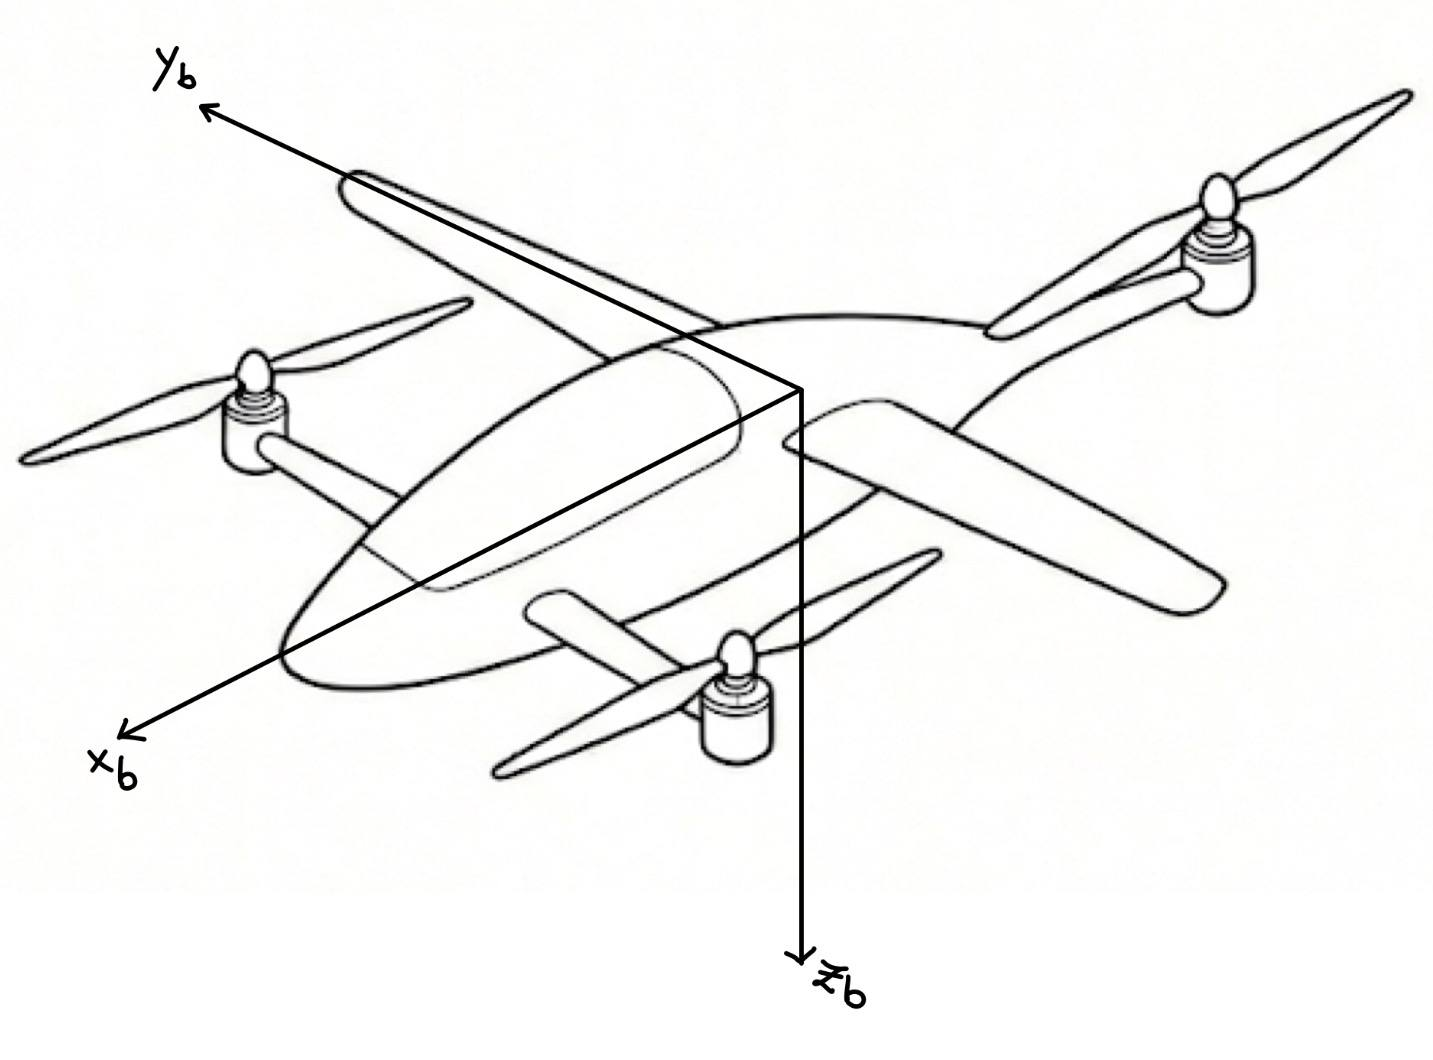
\includegraphics[height=3cm]{sist_rif_body.jpg}
                        \captionof{figure}{Sistema solidale al corpo.}
                    \end{center}
            \end{itemize}
        \end{column}
    \end{columns}
    
    \vspace{0.1cm}
    \textbf{Cinematica (Relazione tra i sistemi):}
    \begin{equation}
        \begin{bmatrix} \bm{\dot{P}}_g \\ \bm{\dot{\Theta}}_g \end{bmatrix} = 
        \begin{bmatrix} \mathbf{R}_{b \to g}(\bm{\Theta}) & \mathbf{0} \\ \mathbf{0} & \mathbf{J}_{b \to g}(\bm{\Theta}) \end{bmatrix}
        \begin{bmatrix} \bm{V}_b \\ \bm{\Omega}_b \end{bmatrix}
    \end{equation}
\end{frame}

% --- SLIDE 2: CONFIGURAZIONE E PROBLEMA ---
% Focus sull'accoppiamento geometrico
\begin{frame}{Configurazione Geometrica e Attuazione}
    \begin{columns}[c]
        \begin{column}{0.5\textwidth}
            \centering
            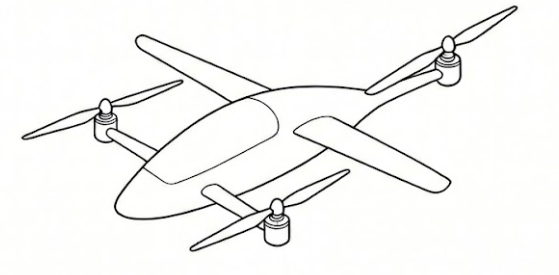
\includegraphics[width=0.9\linewidth]{tricopter_2D.png}
            \captionof{figure}{Configurazione rotori avanzati ($d_x > 0$).}
        \end{column}
        
        \begin{column}{0.5\textwidth}
            \textbf{Configurazione:}
            \begin{itemize}
                \item Rotori Anteriori: $\bm{r}_{1,2} = [d_{mx}, \pm d_{my}, 0]^T$
                \item Rotore di Coda: $\bm{r}_3 = [-d_{tx}, 0, 0]^T$
            \end{itemize}
            
            \vspace{0.5cm}
            \begin{alertblock}{Criticità Dinamica}
                La spinta totale non è applicata nel CoM. 
                \textbf{Implicazione:} Il bilanciamento del \textit{Pitch} richiede una ripartizione di potenza asimmetrica tra rotori anteriori e posteriori.
            \end{alertblock}
        \end{column}
    \end{columns}
\end{frame}

% --- SLIDE 3: NEWTON-EULERO ---
% Forma vettoriale compatta, molto più elegante
\begin{frame}{Equazioni della Dinamica: Newton-Eulero}
    Il modello del corpo rigido è descritto dalle equazioni cardinali nel \textit{Body Frame}:
    
    \vspace{0.5cm}
    \begin{block}{Dinamica Traslazionale e Rotazionale}
    \begin{equation}
        \begin{cases}
            m \bm{\dot{V}}_b = \bm{F}_{\text{tot}} - \underbrace{\bm{\Omega}_b \times (m \bm{V}_b)}_{\text{Coriolis}} \\
            \mathbf{I}_b \bm{\dot{\Omega}}_b = \bm{M}_{\text{tot}} - \underbrace{\bm{\Omega}_b \times (\mathbf{I}_b \bm{\Omega}_b)}_{\text{Giroscopico Body}}
        \end{cases}
    \end{equation}
    \end{block}
    
    \vspace{0.5cm}
    \textbf{Scomposizione delle Forze e Momenti:}
    \begin{itemize}
        \item $\bm{F}_{\text{tot}} = \bm{F}_{\text{th}} + \bm{F}_g + \bm{F}_{\text{aero}}$
        \item $\bm{M}_{\text{tot}} = \bm{M}_{\text{th}} + \bm{M}_{\text{tor}} + \bm{M}_{\text{aero}} + \bm{M}_{\text{gyro}} + \bm{M}_{\text{pinna}}$
    \end{itemize}
\end{frame}

% --- SLIDE 4: FORZE ESTERNE ---
% Condensata: Spinta e Aerodinamica insieme
\begin{frame}{Analisi delle Forze}
    \begin{columns}[T]
        \begin{column}{0.5\textwidth}
            \textbf{1. Spinta Motori ($\bm{F}_{th}$)} \\
            Dipende dall'orientamento ($\theta_i$) e velocità ($\omega_i$) dei rotori:
            \begin{equation*}
                \bm{F}_{th} = \sum_{i=1}^3 \mathbf{R}_{rot_i \to b}(\theta_i) \cdot [0, 0, k\omega_i^2]^T
            \end{equation*}
            
            \vspace{0.2cm}
            \textbf{2. Gravità ($\bm{F}_g$)} \\
            Proiezione del vettore peso:
            \begin{equation*}
                \bm{F}_g = \mathbf{R}_{g \to b} \cdot [0, 0, mg]^T
            \end{equation*}
        \end{column}
        
        \begin{column}{0.5\textwidth}
            \textbf{3. Aerodinamica ($\bm{F}_{aero}$)} \\
            Modello non-lineare per fusoliera e ali:
            \begin{equation*}
                \bm{F}_{wing} \propto \frac{1}{2}\rho S v^2 \cdot \begin{bmatrix} C_D(\alpha) \\ 0 \\ C_L(\alpha) \end{bmatrix}
            \end{equation*}
            \vspace{0.1cm}
            \centering
            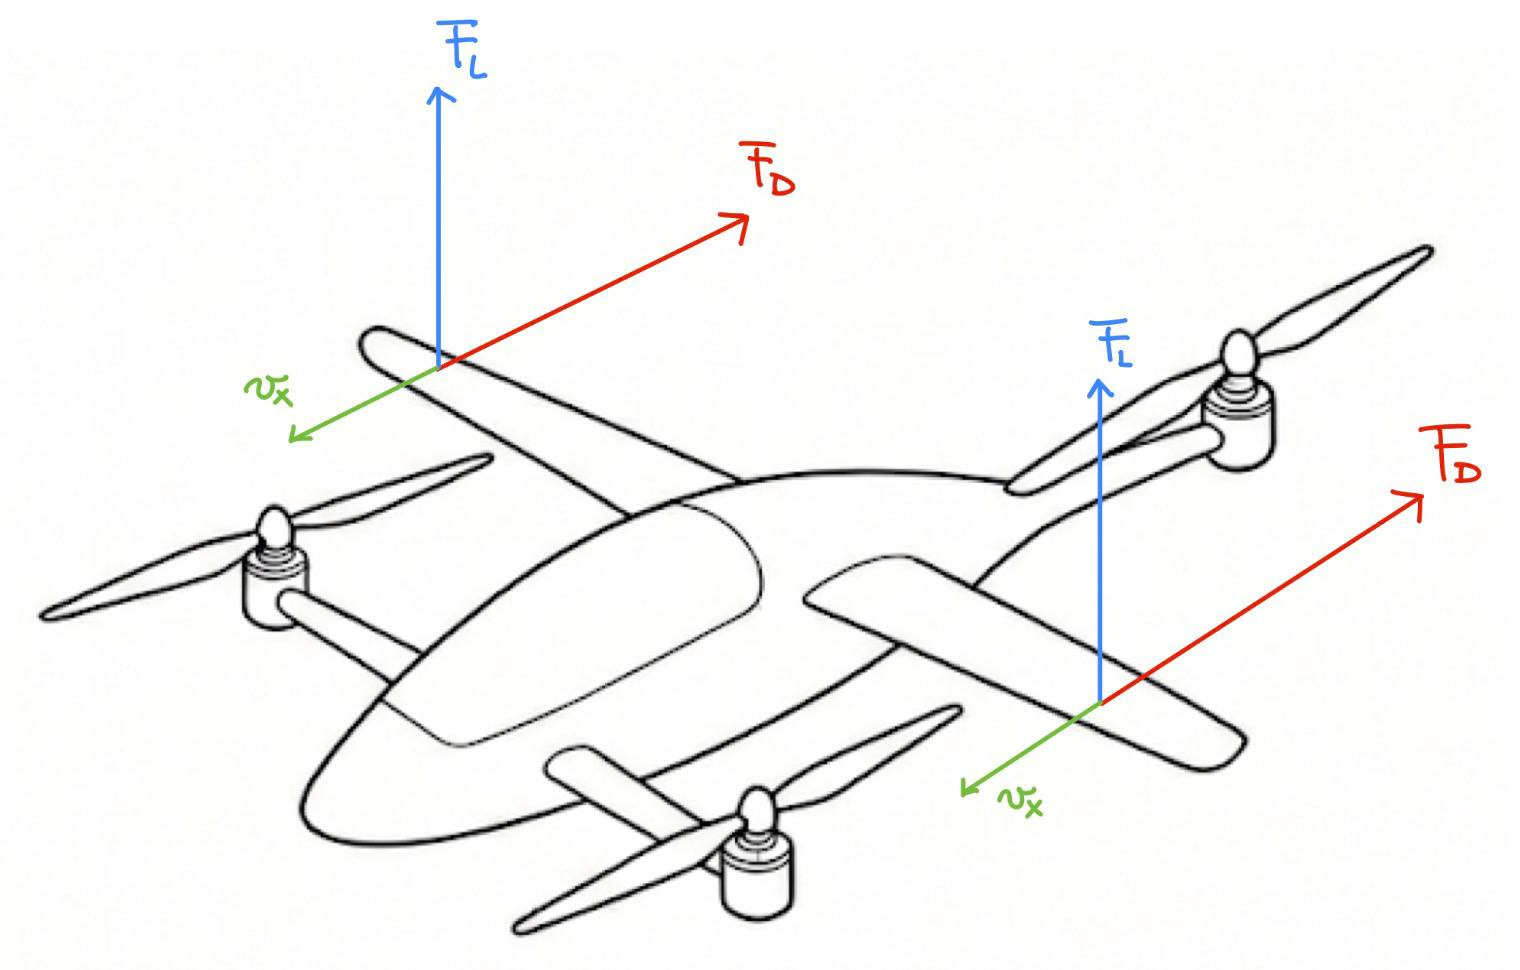
\includegraphics[width=0.8\linewidth]{forze_x.jpg}
        \end{column}
    \end{columns}
\end{frame}

% --- SLIDE 5: MOMENTI ATTIVI (Thrust & Torque) ---
% Raggruppa le slide 16 e 17 originali
\begin{frame}{Momenti Attivi: Controllo del Velivolo}
    I momenti di controllo sono generati dalla combinazione di spinta e reazione dei rotori.
    
    \vspace{0.3cm}
    \textbf{1. Momento di Spinta ($\bm{M}_{th}$)}
    \begin{equation}
        \bm{M}_{\text{th}} = \sum_{i=1}^{3} (\bm{r}_i \times \bm{F}_{th_{i}})
    \end{equation}
    \small \textit{Fondamentale per il controllo di Pitch (leve longitudinali) e Roll (leve laterali).}
    
    \vspace{0.4cm}
    \textbf{2. Momento Torcente ($\bm{M}_{tor}$)}
    \begin{equation}
        \bm{M}_{\text{tor}} = \sum_{i=1}^{3} (b \omega_i^2 + I_{rot} \dot{\omega}_i) \hat{e}_{thrust,i}
    \end{equation}
    \small \textit{La reazione di Drag delle eliche contribuisce principalmente all'imbardata (Yaw).}
\end{frame}

% --- SLIDE 6: MOMENTI REATTIVI (Giroscopico & Pinna) ---
% Raggruppa le slide 19, 20, 21 originali. 
% ELIMINATA la matrice gigante del giroscopico tilting a favore della forma vettoriale.
\begin{frame}{Momenti Reattivi e Dinamica Veloce}
    Effetti dinamici dovuti alla rotazione dei componenti e alla stabilizzazione passiva.

    \begin{block}{Effetto Giroscopico dei Rotori (Tilting)}
        Nasce dalla variazione dell'asse di rotazione dei propulsori ($\bm{\omega}_{tilt}$):
        \begin{equation}
             \bm{M}_{\text{giro}} = \sum_{i=1}^{3} \mathbf{J}_{r} (\bm{\omega}_{\text{tilt},i} \times \bm{\omega}_{r,i})
        \end{equation}
        \footnotesize \textcolor{gray}{(Introduce accoppiamenti forti durante le manovre di transizione rapide)}
    \end{block}

    \vspace{0.3cm}
    \begin{columns}[c]
        \begin{column}{0.5\textwidth}
            \textbf{Momento Pinna di Coda:}
            \begin{equation*}
                M_{z, pinna} \propto -r \cdot v_y^2
            \end{equation*}
            Smorzamento naturale sull'asse di imbardata.
        \end{column}
        \begin{column}{0.5\textwidth}
             \textbf{Giroscopico Body:}
             \begin{equation*}
                 \bm{\Omega}_b \times (\mathbf{I}_b \bm{\Omega}_b)
             \end{equation*}
             Accoppiamento inerziale tra gli assi (es. Roll-Yaw).
        \end{column}
    \end{columns}
\end{frame}

% ==========================================================
% 3. SISTEMA DINAMICO (RIELABORATO)
% ==========================================================
\section{Sistema Dinamico}

\begin{frame}
    \vfill
    \centering
    {\Huge \textbf{Sistema Dinamico e Spazio di Stato}}
    \vfill
\end{frame}

% --- SLIDE 1: FORMULAZIONE DELLO STATO ---
% Unisce definizione e variabili in una sola visione d'insieme potente
\begin{frame}{Formulazione nello Spazio di Stato}
    Il modello è tradotto in un sistema di ODE del tipo $\dot{\mathbf{x}} = f(\mathbf{x}, \mathbf{u}, t)$.
    
    \vspace{0.5cm}
    \textbf{Vettore di Stato ($\mathbf{x} \in \mathbb{R}^{26}$):}
    \begin{equation}
        \mathbf{x} = 
        {
            \renewcommand{\arraystretch}{1.2}
        \begin{bmatrix}
            \bm{P}_g \\ \bm{V}_b \\ \hline
            \bm{\Theta}_g \\ \bm{\Omega}_b \\ \hline
            \bm{\theta}_{rot} \\ \bm{\dot{\theta}}_{rot} \\ \hline
            \bm{\omega}_{rot} \\ \bm{\dot{\omega}}_{rot}
        \end{bmatrix}
        }
        \begin{array}{l}
            \left. \begin{matrix} \text{Posizione Inerziale } [x,y,z] \\ \text{Velocità Body } [u,v,w] \end{matrix} \right\} \text{\textbf{Traslazione}} \\[1em]
            \left. \begin{matrix} \text{Assetto Eulero } [\phi,\theta,\psi] \\ \text{Velocità Angolari } [p,q,r] \end{matrix} \right\} \text{\textbf{Rotazione}} \\[1em]
            \left. \begin{matrix} \text{Posizione Servi} \\ \text{Velocità Servi} \end{matrix} \right\} \text{\textbf{Dinamica Servi}} \\[1em]
            \left. \begin{matrix} \text{Velocità Rotori} \\ \text{Accel. Rotori} \end{matrix} \right\} \text{\textbf{Propulsione}}
        \end{array}
    \end{equation}
\end{frame}

% --- SLIDE 2: INGRESSI DI CONTROLLO ---
% Più pulita, usa colonne per separare logica e matematica
\begin{frame}{Ingressi di Controllo ($\mathbf{u} \in \mathbb{R}^7$)}
    Il vettore degli ingressi $\mathbf{u}$ gestisce sia la potenza che la geometria del velivolo.

    \vspace{0.5cm}
    \begin{columns}[c]
        \begin{column}{0.4\textwidth}
            \centering
            \begin{equation*}
                \mathbf{u} = \begin{bmatrix} 
                u_1 \\ u_2 \\ u_3 \\ \hline
                u_4 \\ u_5 \\ u_6 \\ \hline
                u_7 
                \end{bmatrix}
            \end{equation*}
        \end{column}

        \begin{column}{0.6\textwidth}
            \begin{itemize}
                \item[] \textbf{Propulsione (RPM)}
                \begin{itemize}
                    \item[$u_{1-3}$:] Velocità angolari target ($\omega_{ref}$) per i tre motori.
                \end{itemize}
                \vspace{0.3cm}
                \item[] \textbf{Vettorizzazione (Tilt Anteriore)}
                \begin{itemize}
                    \item[$u_{4-6}$:] Angoli di tilt target per rotori anteriori (attorno a $Y_b$).
                \end{itemize}
                \vspace{0.3cm}
                \item[] \textbf{Yaw Control (Tilt Coda)}
                \begin{itemize}
                    \item[$u_7$:] Angolo di tilt rotore di coda (attorno a $Z_b$).
                \end{itemize}
            \end{itemize}
        \end{column}
    \end{columns}
\end{frame}

% --- SLIDE 3: DINAMICA ATTUATORI ---
% Questa è la slide critica. Sostituisce la cinematica standard con la dinamica realistica
\begin{frame}{Dinamica degli Attuatori}
    È inclusa la dinamica del \textbf{secondo ordine} per motori e servomotori.
    
    \vspace{0.5cm}
    \begin{block}{Modello Dinamico (Esempio per il Tilt $\theta_i$)}
    Ogni attuatore è modellato come un sistema massa-molla-smorzatore:
    \begin{equation}
        \ddot{x}_{servo} = \underbrace{-2\zeta \omega_n \dot{x}_{servo}}_{\text{Smorzamento}} + \underbrace{\omega_n^2 (u_{cmd} - x_{servo})}_{\text{Inseguimento Errore}}
    \end{equation}
    \end{block}

    \vspace{0.5cm}
    \textbf{Implicazioni per il Controllo:}
    \begin{itemize}
        \item Introduce ritardi di fase nella risposta.
        \item Richiede che il controllore di assetto (Inner Loop) sia sufficientemente robusto ai ritardi degli attuatori.
        \item $\zeta \approx 0.7$ (Smorzamento critico), $\omega_n$ identificata sperimentalmente.
    \end{itemize}
\end{frame}


% ============================================================
% 3. ARCHITETTURA DI CONTROLLO (RIELABORATA)
% ============================================================
\section{Architettura di Controllo Verticale}

\begin{frame}
    \vfill
    \centering
    {\Huge \textbf{Controllo Verticale}}
    \vfill
\end{frame}

% --- SLIDE 1: CONFIGURAZIONE & EQUILIBRIO (UNIFICATE) ---
\begin{frame}{Configurazione di Hovering ed Equilibrio}
    In fase di decollo, i rotori anteriori sono verticali ($\theta_{1,2} = 90^\circ$).
    
    \vspace{0.3cm}
    \begin{columns}[c]
        \begin{column}{0.6\textwidth}
            \textbf{Problema:} Il rotore di coda genera una coppia di reazione non bilanciata da un controrotore.
            
            \vspace{0.2cm}
            \textbf{Soluzione ($\theta_{3,eq}$):}
            Si inclina il rotore di coda per generare una componente di spinta laterale che annulli il momento torcente su $Z$.
            
            \vspace{0.2cm}
            \begin{alertblock}{Angolo di Equilibrio}
            Imponendo $M_z^{tot} = 0$:
            \begin{equation}
                \theta_{3_{eq}} = \arctan\left( -\frac{k \, d_{tx}}{b}\right)
            \end{equation}
            \end{alertblock}
        \end{column}
        
        \begin{column}{0.4\textwidth}
            \centering
            % Qui ci starebbe bene uno schemino vettoriale delle forze in coda
            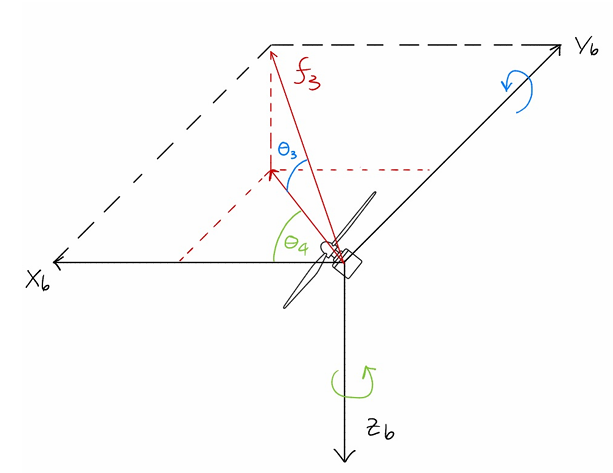
\includegraphics[width=0.8\linewidth]{rotore_3.png} 
            \vspace{0.1cm}
            \captionof{figure}{\footnotesize Compensazione Torque}
        \end{column}
    \end{columns}
\end{frame}

% --- SLIDE 2: PANORAMICA (Invariata nella logica, pulita) ---
\begin{frame}{Architettura Gerarchica a Cascata}
    Si adotta un controllo a cascata per separare la dinamica lenta (traslazione) da quella veloce (rotazione).

    \begin{itemize}
        \item \textbf{Outer Loop (Posizione):} \textcolor{blue}{\textbf{Sliding Mode Control (SMC)}}.
        \begin{itemize}
            \item Robusto ai disturbi esterni (vento).
            \item Genera l'assetto desiderato ($\phi_{des}, \theta_{des}$).
        \end{itemize}
        
        \vspace{0.3cm}
        \item \textbf{Inner Loop (Assetto):} \textcolor{red}{\textbf{PID}}.
        \begin{itemize}
            \item Stabilizza la dinamica angolare veloce.
            \item Genera i momenti richiesti ($M_x, M_y, M_z$).
        \end{itemize}
    \end{itemize}
    
    \vspace{0.5cm}
    \textbf{Sfida Principale:} Accoppiamento forte tra Spinta Totale ($T$) e momento di Beccheggio ($M_y$) dovuto alla geometria asimmetrica.
\end{frame}

% --- SLIDE 3: SCHEMA A BLOCCHI (Il tuo TikZ originale) ---
\begin{frame}{Schema a Blocchi: Volo Verticale}
    \begin{figure}
        \centering
        \resizebox{0.75\textwidth}{!}{
            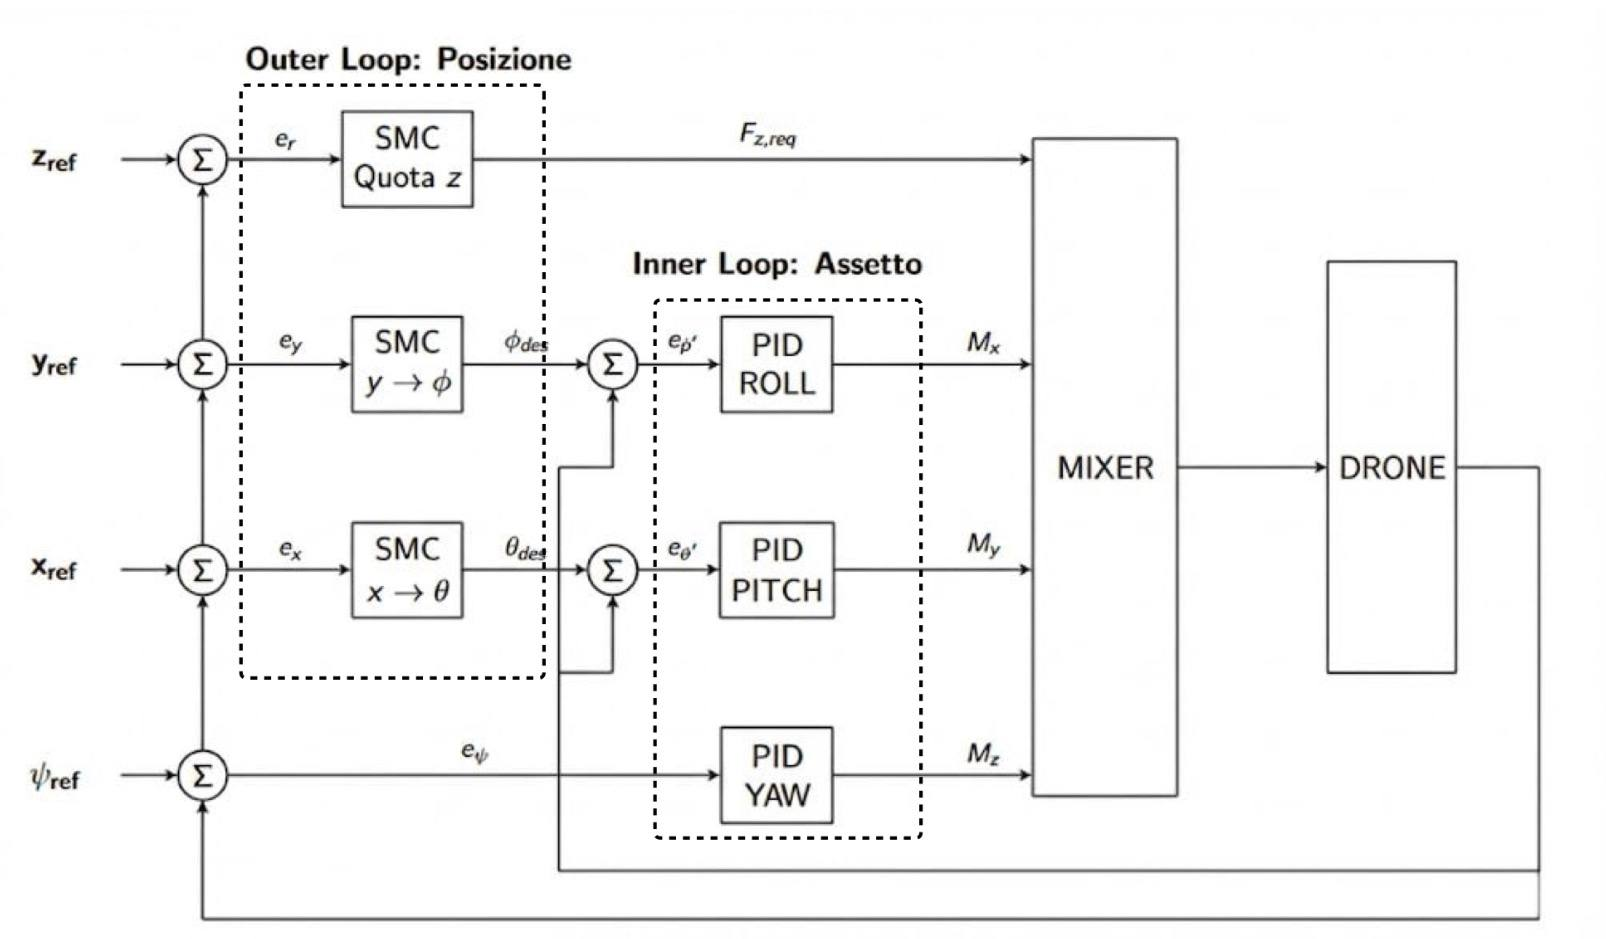
\includegraphics{controllo_verticale/schema_blocchi_V.png}
        }
        \caption{Schema a blocchi del controllo verticale.}
    \end{figure}
\end{frame}

% --- SLIDE 4: SMC QUOTA (INVARIATA) ---
\begin{frame}{Outer Loop: Controllo di Quota}
    \begin{columns}[T]
        \begin{column}{0.6\textwidth}
            \textbf{Obiettivo:} Robustezza ai disturbi.\\
            \vspace{0.2cm}
            \textbf{1. Definizioni:}
            \begin{itemize}
                \item Errore: $e_z = z_{des} - z$
                \item Sliding surface: $\sigma_z = \dot{e}_z + \lambda_z e_z$
            \end{itemize}
            \vspace{0.3cm}
            \textbf{2. Legge di Controllo ($F_{z,req}$):}
            \begin{equation*}
                 \underbrace{mg + F_{aero,z} - m \lambda_z \dot{e}_z}_{\text{Linearizzazione}} - \underbrace{m K_z \tanh\left(\frac{\sigma_z}{\Phi}\right)}_{\text{Termine Robusto}}
            \end{equation*}
            \small
            L'uso di $\tanh(\cdot)$ al posto di $\text{sgn}(\cdot)$ definisce un \textit{boundary layer} $\Phi$ per eliminare il \textit{chattering}.
        \end{column}
        \begin{column}{0.4\textwidth}
            \centering
            \vspace{0.5cm}
            \begin{tikzpicture}[scale=0.8, >=latex]
                \draw[->] (-2,0) -- (2,0) node[right] {$\sigma$};
                \draw[->] (0,-1.5) -- (0,1.5) node[above] {$u_{rob}$};
                \draw[red, dashed, thick] (-1.8,-1) -- (0,-1) -- (0,1) -- (1.8,1);
                \node[red, font=\scriptsize] at (1.5, 1.2) {sgn};
                \draw[blue, thick, domain=-1.8:1.8, samples=50] plot (\x, {tanh(2*\x)});
                \node[blue, font=\scriptsize] at (1.5, 0.6) {tanh};
                \draw[<->, gray] (-0.5, -0.2) -- (0.5, -0.2);
                \node[gray, below, font=\tiny] at (0, -0.2) {$\Phi$};
            \end{tikzpicture}
            \captionof{figure}{\footnotesize Smoothing dell'azione di controllo.}
        \end{column}
    \end{columns}
\end{frame}

% --- SLIDE 5: STABILITÀ (INVARIATA) ---
\begin{frame}{Analisi di Stabilità}
    Per garantire la stabilità asintotica globale della \textit{sliding surface} ($\sigma \to 0$), si utilizza il criterio di Lyapunov.
    \vspace{0.3cm}
    \begin{columns}[T]
        \begin{column}{0.6\textwidth}
            \textbf{1. Funzione Candidata:}
            \begin{equation*}
                V(\sigma) = \frac{1}{2}\sigma^2 > 0
            \end{equation*}
            \textbf{2. Derivata Temporale:}
            Sostituendo la dinamica a ciclo chiuso con disturbo $\Delta$:
            \begin{align*}
                \dot{V} &= \sigma \dot{\sigma} \\
                        &= -k \sigma \text{sgn}(\sigma) + \sigma \Delta \\
                        &\le -k |\sigma| + |\sigma| \delta_{\max}
            \end{align*}
        \end{column}
        \begin{column}{0.4\textwidth}
            \centering
            \vspace{1cm}
            \begin{alertblock}{Condizione di Stabilità}
                Affinché la funzione decresca ($\dot{V} < 0$), il guadagno deve "battere" il disturbo:
                \vspace{0.2cm}
                \centering
                \large
                \boldmath
                $k > \delta_{\max}$
                \unboldmath
            \end{alertblock}
            \small \itshape
            Il sistema è robusto se il guadagno di switching supera il limite superiore dell'incertezza.
        \end{column}
    \end{columns}
\end{frame}

% --- SLIDE 6: GUADAGNI E DISTURBI (INVARIATA) ---
\begin{frame}{Gestione dei Disturbi e Tuning del Guadagno}
    Il vantaggio principale dello SMC è che non richiede la conoscenza puntuale del disturbo $d(t)$, ma solo del suo upper bound.
    \begin{columns}[c]
        \begin{column}{0.5\textwidth}
            \textbf{Condizione di Robustezza:}
            $$ k > |\Delta(t)|_{\max} $$
            \small
            \begin{itemize}
                \item \textcolor{green!60!black}{\textbf{Guadagno Ottimale:}} $k$ leggermente superiore al disturbo massimo atteso. Stabilità garantita e chattering ridotto.
                \item \textcolor{red}{\textbf{Guadagno Eccessivo:}} Stabilità garantita, ma forte chattering e stress sugli attuatori.
                \item \textcolor{orange}{\textbf{Guadagno Insufficiente:}} Il disturbo "rompe" il vincolo di sliding. Perdita di stabilità.
            \end{itemize}
        \end{column}
        \begin{column}{0.5\textwidth}
            \centering
            \begin{tikzpicture}[scale=0.8]
                \draw[->] (0,0) -- (5,0) node[right] {$t$};
                \draw[->] (0,-2.5) -- (0,2.5) node[above] {Ampiezza};
                \draw[gray, thick, domain=0:4.5, samples=100] plot (\x, {1.2*sin(deg(\x*3)) + 0.5*sin(deg(\x*10))});
                \node[gray, right] at (4.5, -0.5) {$d(t)$};
                \draw[dashed, red] (0, 1.8) -- (4.5, 1.8);
                \draw[dashed, red] (0, -1.8) -- (4.5, -1.8);
                \node[red, font=\tiny] at (0.5, 1.9) {$\delta_{max}$};
                \draw[blue, thick] (0, 2.0) -- (4.5, 2.0) node[right] {$k_{buono}$};
                \draw[blue, thick] (0, -2.0) -- (4.5, -2.0);
                \fill[blue, opacity=0.1] (0,-2) rectangle (4.5,2);
            \end{tikzpicture}
            \captionof{figure}{\footnotesize Il guadagno $k$ (blu) deve contenere il disturbo (grigio).}
        \end{column}
    \end{columns}
\end{frame}

% --- SLIDE 7: INVERSIONE DINAMICA (Semplificata) ---
\begin{frame}{Controllo Planare: Inversione Cinematica}
    Le forze virtuali calcolate dagli SMC ($F_{x,req}, F_{y,req}$) sono convertite in angoli di assetto desiderati.
    
    \vspace{0.5cm}
    \begin{columns}[c] % [c] allinea verticalmente al centro. Usa [T] solo se necessario.
    % Prima colonna: ridotta al 48% per lasciare spazio al centro
        \begin{column}{0.48\textwidth}
            \begin{block}{Generazione Rollio ($\phi_{des}$)}
                \begin{equation*}
                    \phi_{des} = \arcsin\left( \frac{F_{y,req}}{T} \right)
                \end{equation*}
                Compensa l'errore laterale $e_y$.
            \end{block}
        \end{column}
        
        % Spazio elastico che spinge le colonne agli estremi
        \hfill 
        
        % Seconda colonna: ridotta al 48%
        \begin{column}{0.48\textwidth}
            \begin{block}{Generazione Beccheggio ($\theta_{des}$)}
                \begin{equation*}
                    \theta_{des} = \arcsin\left( - \frac{F_{x,req}}{T} \right)
                \end{equation*}
                Compensa l'errore longitudinale $e_x$.
            \end{block}
        \end{column}
    \end{columns}
    
    \vspace{0.5cm}
    \textbf{Inner Loop (Attitude):}
    L'inseguimento degli angoli è affidato a tre controllori \textbf{PID} standard che generano i momenti richiesti:
    \begin{equation*}
        \mathbf{M}_{req} = K_P \cdot \mathbf{e}_{ang} + K_I \int \mathbf{e}_{ang} + K_D \cdot \dot{\mathbf{e}}_{ang}
    \end{equation*}
\end{frame}

% --- SLIDE 8: MMA Longitudinale (Condensata) ---
\begin{frame}{Motor Mixing Algorithm: Longitudinale}
    La dinamica longitudinale richiede la risoluzione di un sistema accoppiato: Spinta ($T$) e Beccheggio ($M_y$).
    
    \vspace{0.3cm}
    \textbf{1. Calcolo Rotore di Coda ($\omega_3$):}
    Dall'equilibrio dei momenti attorno a Y, si isola il contributo della coda:
    \begin{equation}
        \omega_3^2 = \frac{M_y - F_{z,req} d_{mx}}{k \sin(\theta_3) (d_{tx} - d_{mx}) + b \cos(\theta_3) \sin(\theta_4)}
    \end{equation}
    
    \vspace{0.3cm}
    \textbf{2. Calcolo Rotori Anteriori ($T_{front}$):}
    Nota la spinta della coda, il resto del sostentamento è affidato al fronte:
    \begin{equation}
        T_{front} = F_{z,req} - T_3 \sin(\theta_3)
    \end{equation}
\end{frame}

% --- SLIDE 9: MMA Laterale (Condensata) ---
\begin{frame}{Motor Mixing Algorithm: Latero-Direzionale}
    Una volta determinato $T_{front}$, questo viene modulato per controllare Roll e Yaw.
    
    \vspace{0.5cm}
    \begin{columns}[T]
        \begin{column}{0.5\textwidth}
            \textbf{ROLL (Spinta Differenziale)} \\
            Si ripartisce la spinta anteriore tra destra ($T_1$) e sinistra ($T_2$):
            \begin{equation*}
                T_{1,2} = \frac{T_{front}}{2} \mp \frac{M_x}{2 d_{my}}
            \end{equation*}
        \end{column}
        \begin{column}{0.5\textwidth}
            \textbf{YAW (Tilt Differenziale)} \\
            Si inclina il vettore spinta anteriore per creare coppia su Z:
            \begin{equation*}
                \delta_{des} = \arcsin\left( \frac{M_{z,req}}{T_{front} d_{my}} \right)
            \end{equation*}
            \begin{itemize}
                \item $\theta_1 = 90^\circ - \delta_{des}$
                \item $\theta_2 = 90^\circ + \delta_{des}$
            \end{itemize}
        \end{column}
    \end{columns}
\end{frame}

% ===========================================================
% SIMULAZIONI (RIELABORATE)
% ==========================================================
\section{Simulazioni controllo verticale}

\begin{frame}
    \vfill
    \centering
    {\Huge \textbf{Risultati Simulazione}}
    \vfill
\end{frame}

% --- SLIDE SIMULAZIONI 1: Assetto ---
\begin{frame}{Analisi Prestazionale: Assetto e Posizione}
    \begin{columns}[c]
        \begin{column}{0.65\textwidth}
            \centering
            
\includegraphics[width=\linewidth]{angoli.png}
        \end{column}
        \begin{column}{0.35\textwidth}
            \textbf{Risposta Angolare:}
            \begin{itemize}
                \item \textcolor{blue!80!black}{\textbf{Velocità:}} Settling time < 2s.
                \item \textcolor{blue!80!black}{\textbf{Precisione:}} Errore a regime nullo sugli angoli di Eulero.
                \item \textcolor{blue!80!black}{\textbf{Overshoot:}} Minimo (< 5\%) durante i transitori.
            \end{itemize}
        \end{column}
    \end{columns}
\end{frame}

% --- SLIDE SIMULAZIONI 2: Attuatori ---
\begin{frame}{Analisi degli Attuatori: Sforzo di Controllo}
    \begin{columns}[c]
        \begin{column}{0.65\textwidth}
            
\includegraphics[width=\linewidth]{thrust.png}
            \vspace{0.1cm}
            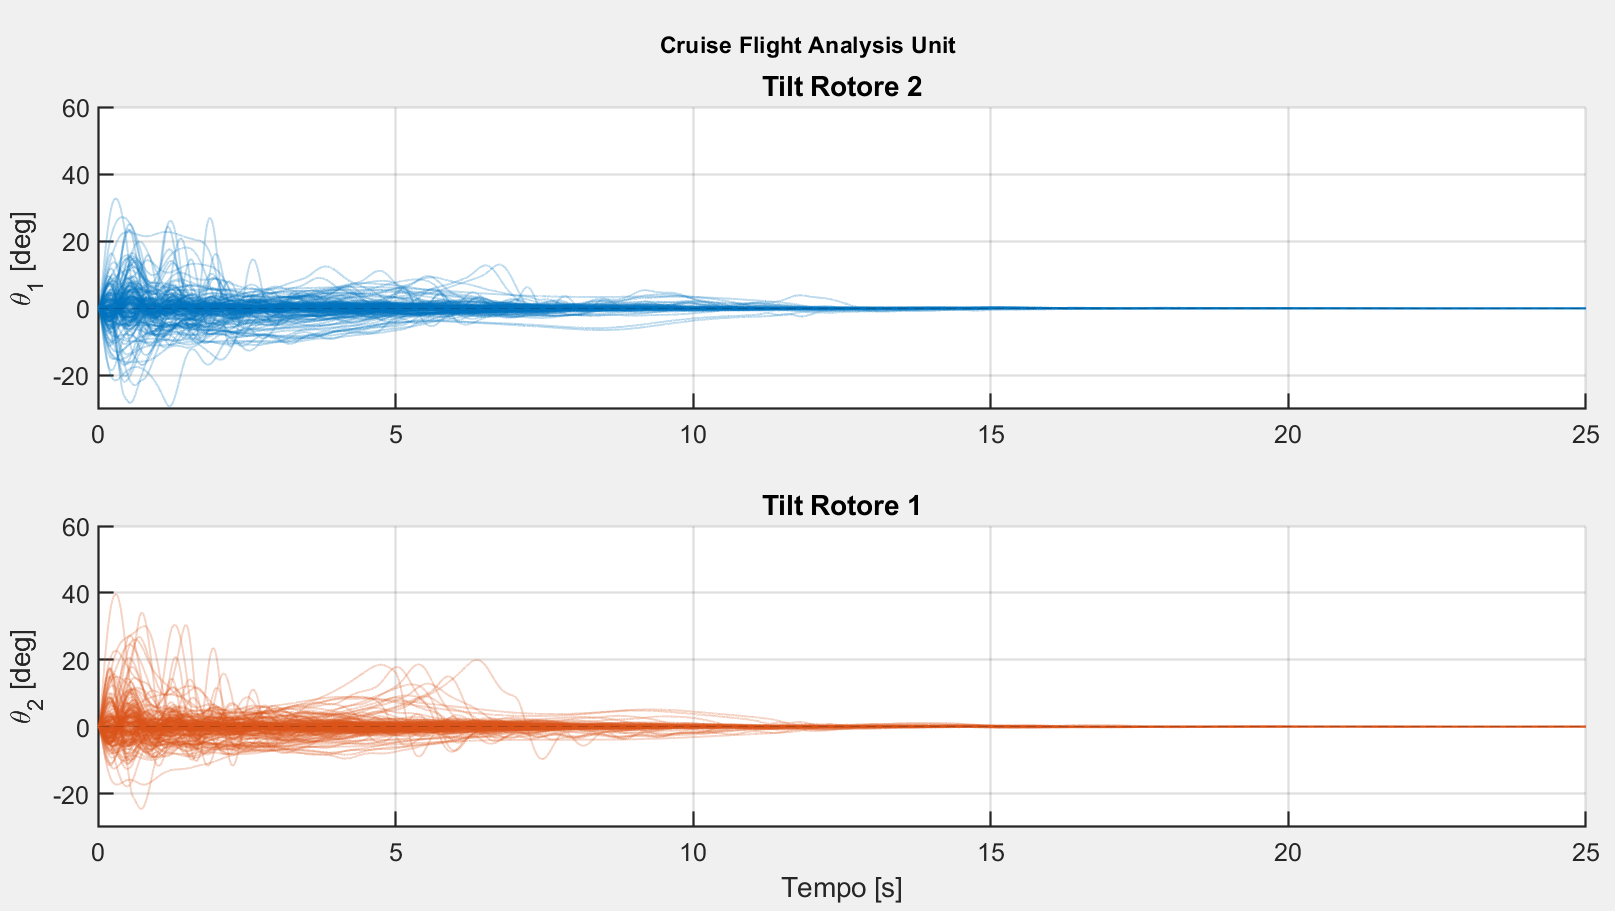
\includegraphics[width=\linewidth]{tilt.png}
        \end{column}
        \begin{column}{0.35\textwidth}
            \textbf{Thrust:}
            \begin{itemize}
                \item Nessuna saturazione dei motori (Max 100N).
                \item \textit{Ripple} limitato all'ingresso dei disturbi.
            \end{itemize}
            \vspace{0.5cm}
            \textbf{Tilt:}
            \begin{itemize}
                \item Escursione contenuta ($\pm 5^\circ$) in hovering.
                \item Dinamica compatibile con la banda passante dei servi.
            \end{itemize}
        \end{column}
    \end{columns}
\end{frame}

% ===========================================================
% MONTECARLO HOVERING
% ===========================================================
% \begin{frame}
%     \vfill
%     \centering
%     {\Huge \textbf{Analisi di Monte Carlo per il volo verticale}}
%     \vfill
% \end{frame}

% % --- Slide 2: Setup Sperimentale ---
% \begin{frame}{Setup Monte Carlo: Recovery Test}
%     Test di recupero da condizioni iniziali degradate ($N=100$ run).
%     \vspace{0.3cm}
%     \begin{itemize}
%         \item \textbf{Target:} Punto fisso $[0, 0, -10]$ \si{\meter}.
%         \item \textbf{Perturbazioni (Uniformi):}
%         \begin{itemize}
%             \item \textbf{Posizione Planare (X, Y):} $\pm \SI{5}{\meter}$.
%             \item \textbf{Quota (Z):} $[-15, -5]$ \si{\meter}.
%             \item \textbf{Assetto:} $\phi, \theta \in [-20^\circ, +20^\circ]$ (Stress test).
%         \end{itemize}
%     \end{itemize}
%     \vspace{0.2cm}
%     \textit{Obiettivo: Validare la capacità di raggiungimento del target da condizioni iniziali sfavorevoli.}
% \end{frame}

% % --- Slide 3: Robustezza Totale ---
% \begin{frame}{Statistiche di Convergenza}
%     \begin{center}
%         \begin{beamerboxesrounded}[upper=block title, lower=block body, shadow=true]{Risultato Globale}
%             \centering
%             \huge \textbf{Success Rate: 100\%}
%         \end{beamerboxesrounded}
%     \end{center}
%     \vspace{0.3cm}
%     \begin{itemize}
%         \item \textbf{Sicurezza:} Nessun crash registrato su 100 tentativi estremi.
%         \item \textbf{Stabilità:} Il sistema recupera l'assetto anche partendo da $20^\circ$ di inclinazione.
%     \end{itemize}
% \end{frame}

% % --- Slide 4: Precisione Planare (X vs Y) ---
% \begin{frame}{Analisi Differenziale Assi Planari (X, Y)}
%     Emergono comportamenti dinamici diversi tra il canale Longitudinale (X) e Laterale (Y).
    
%     \vspace{0.2cm}
%     \begin{table}
%         \centering
%         \small
%         \begin{tabular}{lcccc}
%             \toprule
%             \textbf{Canale} & \textbf{RMSE Mediana} & \textbf{RMSE Medio} & \textbf{Max Error} & \textbf{Comportamento} \\
%             \midrule
%             \textbf{Laterale (Y)} & \SI{2.2}{\centi\meter} & \SI{2.2}{\centi\meter} & \SI{2.2}{\centi\meter} & \textcolor{blue}{Consistente} \\
%             \textbf{Longit. (X)} & \cellcolor{green!20}$\mathbf{< \SI{10}{\micro\meter}}$ & \cellcolor{red!10}\SI{5.48}{\meter} & \SI{135}{\meter} & \textcolor{red}{Bimodale} \\
%             \bottomrule
%         \end{tabular}
%     \end{table}
    
%     \begin{alertblock}{Risultati}
%         \begin{itemize}
%             \item \textbf{Caso Tipico (75\% dei casi):} Il controllo su X è \textbf{efficace} (errori in $\mu m$), superiore alla Y.
%             \item \textbf{Outliers (25\% dei casi):} In condizioni specifiche (es. pitch iniziale opposto al target), il drone satura e "slitta" (drift) accumulando errore metrico.
%         \end{itemize}
%     \end{alertblock}
% \end{frame}

% % --- Slide 5: Precisione Verticale (Z) ---
% \begin{frame}{Performance Canale Verticale (Z)}
%     Il mantenimento della quota è robusto e disaccoppiato dalle problematiche planari.
    
%     \vspace{0.3cm}
%     \begin{columns}
%         \begin{column}{0.5\textwidth}
%             \begin{itemize}
%                 \item \textbf{RMSE Medio:} \SI{7.7}{\ milli\meter}
%                 \item \textbf{RMSE Mediana:} $< \SI{1}{\micro\meter}$
%                 \item \textbf{Max Error:} \SI{17}{\centi\meter}
%             \end{itemize}
%         \end{column}
%         \begin{column}{0.5\textwidth}
%             \begin{block}{Valutazione}
%                 Eccellente. Anche nei casi di "drift" planare su X, la quota viene mantenuta perfettamente. Questo conferma un buon disaccoppiamento nel design del controllore.
%             \end{block}
%         \end{column}
%     \end{columns}
% \end{frame}

% % --- Slide 6: Analisi Ratei (La Causa del Drift) ---
% \begin{frame}{Analisi Sforzo Attuatori (Inner Loop)}
%     Perché la X ha degli outliers? Guardiamo i ratei richiesti.
    
%     \vspace{0.2cm}
%     \begin{table}
%         \centering
%         \small
%         \begin{tabular}{lccc}
%             \toprule
%             \textbf{Asse} & \textbf{Attività Media (RMSE)} & \textbf{Picco Max} & \textbf{Stress} \\
%             \midrule
%             Roll ($p$) & $\approx 0$ & $3 \times 10^{-4}$ & Nullo \\
%             Yaw ($r$) & $\approx 0$ & $2 \times 10^{-4}$ & Nullo \\
%             \rowcolor{yellow!20}\textbf{Pitch ($q$)} & \textbf{\SI{0.025}{rad/s}} & \textbf{\SI{0.55}{rad/s}} & \textbf{Alto} \\
%             \bottomrule
%         \end{tabular}
%     \end{table}
    
%     \textbf{Conclusione Tecnica:}
%     Il canale di Pitch lavora sotto stress elevato (picchi di \SI{31}{\degree\per\second}).
%     Gli errori su X nascono quando la richiesta di coppia di pitch eccede la banda passante o l'autorità istantanea dei rotori, causando un ritardo nella frenata.
% \end{frame}

% % --- Slide 7: Sintesi Finale ---
% \begin{frame}{Sintesi Validazione Hovering}
%     \begin{columns}
%         \begin{column}{0.6\textwidth}
%             \textbf{Stato Sistema:}
%             \begin{itemize}
%                 \item[\checkmark] \textbf{Safety:} 100\% Convergenza (Nessun crash).
%                 \item[\checkmark] \textbf{Precisione Nominale:} Eccellente su tutti gli assi ($< 3$cm).
%                 \item[\textbf{!}] \textbf{Limiti:} Tendenza al drift su X (Pitch) in manovre di recupero estreme.
%             \end{itemize}
%         \end{column}
%         \begin{column}{0.4\textwidth}
%             \begin{block}{Roadmap}
%                 Il controllore è \textbf{pronto per il volo} in condizioni nominali.
%                 Si consiglia un tuning più aggressivo del guadagno derivativo (D) sul Pitch per limitare i drift negli outliers.
%             \end{block}
%         \end{column}
%     \end{columns}
% \end{frame}

% ============================================================
% 4. CONTROLLO ORIZZONTALE (RIELABORATO)
% ============================================================
\section{Controllo Volo Orizzontale}

\begin{frame}
    \vfill
    \centering
    {\Huge \textbf{Controllo Orizzontale}}
    \vfill
\end{frame}

% --- SLIDE 1: CONFIGURAZIONE CROCIERA ---
\begin{frame}{Configurazione di Crociera (Fixed-Wing Mode)}
    Durante il volo avanzato, i rotori anteriori generano spinta propulsiva orizzontale.
    
    \vspace{0.3cm}
    \begin{columns}[c]
        \begin{column}{0.6\textwidth}
            \textbf{Configurazione:}
            \begin{itemize}
                \item Rotori Anteriori: $\theta \approx 0^\circ$ (Orizzontali).
                \item Rotore di Coda: \textbf{Spento} (per evitare instabilità su Roll/Yaw).
            \end{itemize}
            
            \vspace{0.3cm}
            \begin{alertblock}{La Sfida di Controllo}
                Il velivolo è \textbf{sotto-attuato} e privo di superfici aerodinamiche mobili (alettoni, flap, timone).
                Tutto il controllo di assetto è affidato al \textbf{Thrust Vectoring} dei soli due rotori anteriori.
            \end{alertblock}
        \end{column}
        
        \begin{column}{0.4\textwidth}
            \centering
            % Placeholder per immagine drone in volo orizzontale
            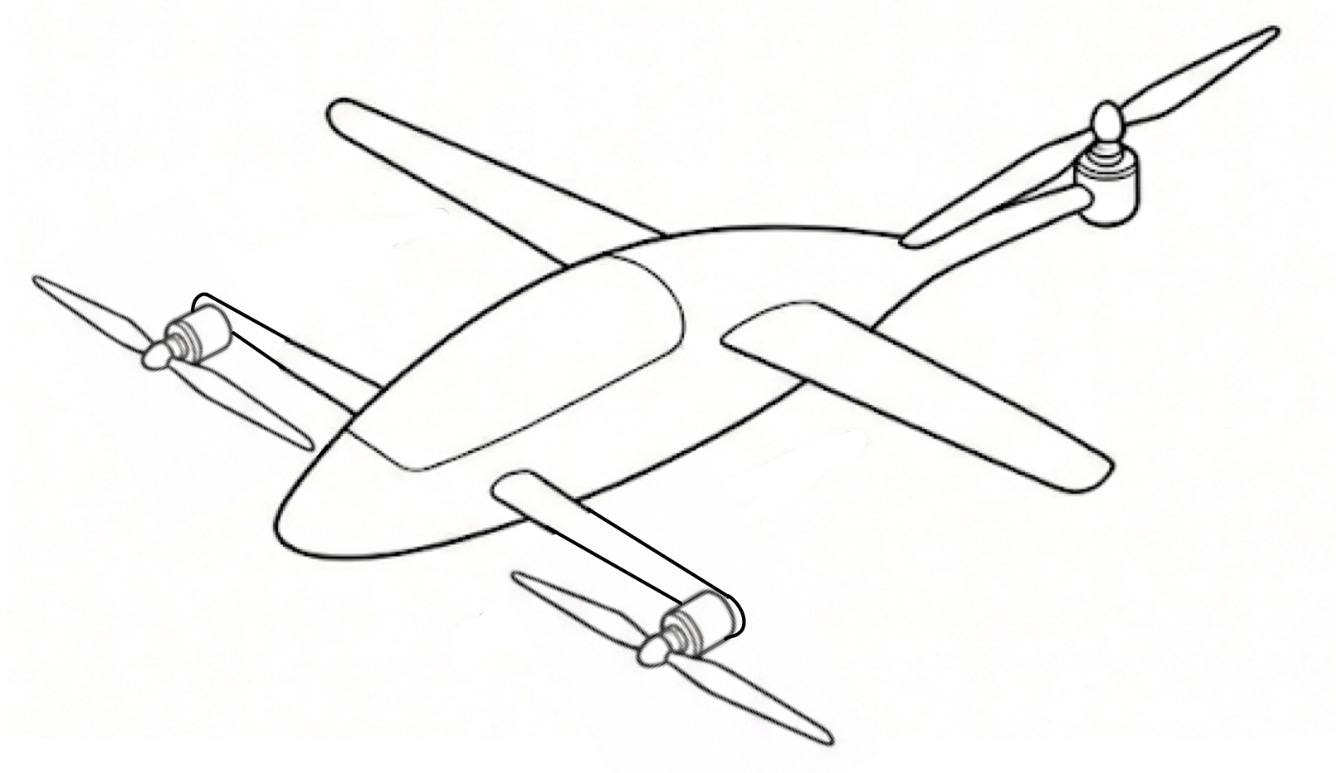
\includegraphics[width=0.9\linewidth]{config_orizzontale.png} 
            \captionof{figure}{\footnotesize Configurazione Forward Flight}
        \end{column}
    \end{columns}
\end{frame}

% --- SLIDE 2: SCHEMA A BLOCCHI (Il tuo TikZ) ---
\begin{frame}{Schema a blocchi: Controllo Orizzontale}
    \begin{figure}[htbp]
    \centering
    \resizebox{0.85\textwidth}{!}{
    \begin{tikzpicture}[auto, node distance=1.3cm, >=Stealth, thick]
        % --- STILI ---
        \tikzset{
            block/.style={draw, rectangle, minimum height=3em, minimum width=4.5em, align=center, fill=white},
            sum/.style={draw, circle, inner sep=0pt, minimum size=6mm},
            input/.style={coordinate},
            output/.style={coordinate},
            container/.style={draw, rectangle, rounded corners, dashed, inner sep=0.4cm}
        }

        % --- COLONNA 1: OUTER LOOP ---
        \node [input] (ref_z) {};
        \node [sum, right=0.8cm of ref_z] (sum_z) {$\Sigma$};
        \node [block, right=1cm of sum_z] (pid_z) {PID\\$z$};
        \node [left=0.1cm of ref_z] {$z_{des}$};

        \node [input, below=1.5cm of ref_z] (ref_vx) {};
        \node [sum, right=0.8cm of ref_vx] (sum_vx) {$\Sigma$};
        \node [block, right=1cm of sum_vx] (pid_vx) {PID\\$v_x$};
        \node [left=0.1cm of ref_vx] {$v_{x,des}$};

        \node [input, below=3.5cm of ref_vx] (ref_y) {};
        \node [sum, right=0.8cm of ref_y] (sum_y) {$\Sigma$};
        \node [block, right=1cm of sum_y] (pid_y) {PID\\$y$};
        \node [left=0.1cm of ref_y] {$y_{des}$};

        % --- COLONNA 2: INNER LOOP ---
        \node [sum, right=3cm of pid_vx, yshift=-1.5cm] (sum_theta) {$\Sigma$};
        \node [block, right=0.8cm of sum_theta] (pid_theta) {PID\\$\theta$};
        
        \node [sum, right=3cm of pid_y] (sum_phi) {$\Sigma$};
        \node [block, right=0.8cm of sum_phi] (pid_phi) {PID\\$\phi$};

        \node [sum, below=1cm of sum_phi] (sum_psi) {$\Sigma$};
        \node [block, right=0.8cm of sum_psi] (pid_psi) {PID\\$\psi$};

        % --- COLONNA 3: MIXER E DRONE ---
        \node [block, right=8.5cm of pid_vx, minimum height=10.5cm, yshift=-2cm] (mixer) {MMA};
        \node [block, right=1.5cm of mixer, minimum height=8.5cm] (drone) {DRONE};
        \node [output, right=1cm of drone] (drone_out) {};

        % --- CONNESSIONI DIRETTE ---
        \draw [->] ($(sum_theta.west)-(0.8,0)$) -- node[above, pos=0] {$\theta_{des}$} (sum_theta.west);
        \draw [->] ($(sum_psi.west)-(0.8,0)$) -- node[above, pos=0] {$r_{des}$} (sum_psi.west);

        \draw [->] (pid_z.east) -- (mixer.west |- pid_z.east) node[above, pos=0.15] {$F_{z,req}$};
        \draw [->] (pid_vx.east) -- (mixer.west |- pid_vx.east) node[above, pos=0.15] {$F_{x,req}$};
        \draw [->] (pid_theta.east) -- (mixer.west |- pid_theta.east) node[above, pos=0.5] {$\theta_{pitch}$};
        \draw [->] (pid_phi.east) -- (mixer.west |- pid_phi.east) node[above, pos=0.5] {$\delta$};
        \draw [->] (pid_psi.east) -- (mixer.west |- pid_psi.east) node[above, pos=0.5] {$\Delta \omega$};

        \draw [->] (ref_z) -- (sum_z); \draw [->] (sum_z) -- (pid_z);
        \draw [->] (ref_vx) -- (sum_vx); \draw [->] (sum_vx) -- (pid_vx);
        \draw [->] (ref_y) -- (sum_y); \draw [->] (sum_y) -- (pid_y);
        \draw [->] (pid_y.east) -- node[above] {$\phi_{des}$} (sum_phi.west);
        \draw [->] (sum_theta) -- (pid_theta);
        \draw [->] (sum_phi) -- (pid_phi);
        \draw [->] (sum_psi) -- (pid_psi);
        \draw [->] (mixer) -- (drone);
        \draw [->] (drone) -- (drone_out);

        % --- FEEDBACK BUS ---
        \coordinate (fb_node) at ($(drone.east)+(0.5,0)$);
        \coordinate (line_outer) at (0,-9.8); % Bus per Outer Loop
        \coordinate (line_inner) at (0,-9);    % Bus per Inner Loop

        \draw (fb_node) |- (line_outer) -- ($(sum_z.west |- line_outer)$);
        \draw (fb_node) |- (line_inner) -- ($(sum_theta.west |- line_inner)$);

        \draw [->, shorten >=0.5pt] (sum_z.south |- line_outer) -- (sum_z.south) node[left, pos=0.85] {$-$};
        \draw [->, shorten >=0.5pt] (sum_vx.south |- line_outer) -- (sum_vx.south) node[left, pos=0.85] {$-$};
        \draw [->, shorten >=0.5pt] (sum_y.south |- line_outer) -- (sum_y.south) node[left, pos=0.85] {$-$};

        \draw [->, shorten >=0.5pt] (sum_theta.south |- line_inner) -- (sum_theta.south) node[left, pos=0.7] {$-$};
        \draw [->, shorten >=0.5pt] (sum_phi.south |- line_inner) -- (sum_phi.south) node[left, pos=0.7] {$-$};
        \draw [->, shorten >=0.5pt] (sum_psi.south |- line_inner) -- (sum_psi.south) node[left, pos=0.85] {$-$};

        % --- CONTAINERS ---
        \begin{scope}[on background layer]
            \node [container, draw, fit=(sum_z) (pid_z) (sum_y) (pid_y), label={above:\textbf{Outer Loop}}] {};
            \node [container, draw, fit=(sum_theta) (pid_theta) (sum_psi) (pid_psi), label={below:\textbf{Inner Loop}}] {};
        \end{scope}

    \end{tikzpicture}
    }
    \caption{Architettura a Cascata: Guidance (Lento) e Attitude (Veloce).}
    \end{figure}
\end{frame}

% --- SLIDE 3: OUTER LOOP (UNIFICATA) ---
\begin{frame}{Outer Loop: Guidance (Quota e Velocità)}
    L'Outer Loop genera le forze richieste ($F_{req}$) per inseguire i riferimenti. Entrambi i canali utilizzano un Feedforward Aerodinamico.
    
    \vspace{0.3cm}
    \begin{columns}[T]
        % Colonna Quota
        \begin{column}{0.48\textwidth}
            \begin{block}{Controllo Quota ($z$)}
                Mantenimento altitudine tramite modulazione forza verticale:
                \begin{equation}
                    F_{z,req} = \underbrace{m (g - a_{z,PID})}_{\text{Inerziale}} - \underbrace{L_{wing}(v)}_{\text{Lift Feedforward}}
                \end{equation}
            \end{block}
        \end{column}
        
        % Colonna Velocità
        \begin{column}{0.48\textwidth}
            \begin{block}{Controllo Velocità ($v_x$)}
                Inseguimento del setpoint ($25 m/s$) tramite forza propulsiva:
                \begin{equation}
                    F_{x,req} = \underbrace{F_{x,PID}}_{\text{Correttivo}} + \underbrace{D_{x}(v)}_{\text{Drag Feedforward}}
                \end{equation}
            \end{block}
        \end{column}
    \end{columns}
    
\end{frame}

% --- SLIDE 4: INNER LOOP (ANALOGIE) ---
\begin{frame}{Inner Loop: Thrust Vectoring come Superfici Virtuali}
    In assenza di alettoni e timoni, il mixer emula le superfici di controllo classiche usando i motori.

    \vspace{0.3cm}
    \begin{columns}[T]
        \begin{column}{0.32\textwidth}
            \begin{alertblock}{Pitch ($\theta$)}
                \centering \textbf{"Elevator"}
                \vspace{0.2cm}
                \begin{itemize}
                    \item \textbf{Azione:} Tilt Collettivo.
                    \item $\theta_1 = \theta_2$.
                    \item Ruota il vettore spinta su/giù.
                \end{itemize}
            \end{alertblock}
        \end{column}

        \begin{column}{0.32\textwidth}
            \begin{block}{Roll ($\phi$)}
                \centering \textbf{"Ailerons"}
                \vspace{0.2cm}
                \begin{itemize}
                    \item \textbf{Azione:} Tilt Differenziale.
                    \item $\theta_1 = -\theta_2$.
                    \item Crea coppia torcente sull'asse $X$.
                \end{itemize}
            \end{block}
        \end{column}

        \begin{column}{0.32\textwidth}
            \begin{exampleblock}{Yaw ($\psi$)}
                \centering \textbf{"Rudder"}
                \vspace{0.2cm}
                \begin{itemize}
                    \item \textbf{Azione:} Spinta Differenziale.
                    \item $T_1 \neq T_2$.
                    \item Crea coppia torcente sull'asse $Z$.
                \end{itemize}
            \end{exampleblock}
        \end{column}
    \end{columns}
\end{frame}

% --- SLIDE 5: MMA CONCETTO (SINTESI VETTORIALE) ---
\begin{frame}{Motor Mixing: Sintesi e Compensazione Geometrica}
    Il Mixer traduce le forze cartesiane ($F_x, F_z$) in un vettore spinta, compensando l'assetto istantaneo del drone.

    \vspace{0.3cm}
    \textbf{1. Sintesi del Vettore Spinta (Frame Inerziale)}
    \begin{equation}
        T_{tot} = \sqrt{F_{x}^2 + F_{z}^2} \quad ; \quad \alpha_{inertial} = \arctan2(F_z, F_x)
    \end{equation}

    \vspace{0.3cm}
    \textbf{2. Trasformazione al Body Frame (Compensazione)}
    I servi sono solidali alla fusoliera. Se il drone cabra ($\theta > 0$), i motori devono ruotare in basso per mantenere la spinta orizzontale.
    
    \begin{equation}
        \boxed{\alpha_{base} = \alpha_{inertial} - \theta_{body}}
    \end{equation}
    
    \small \textit{Questo disaccoppia la dinamica di traslazione dalle oscillazioni di beccheggio.}
\end{frame}

% --- SLIDE 6: MMA ATTUAZIONE (EQUAZIONI FINALI) ---
\begin{frame}{Motor Mixing: Leggi di Attuazione}
    Ai valori di base si sovrappongono i comandi di stabilizzazione ($u_\phi, u_\psi$) dell'Inner Loop.

    \vspace{0.5cm}
    % L'opzione 'onlytextwidth' assicura che il calcolo delle larghezze sia pulito
    \begin{columns}[c, onlytextwidth] 
        \hfill % Margine sinistro (opzionale, per centrare il blocco totale)
        
        \begin{column}{0.44\textwidth}
            \centering % Centra il contenuto dentro la colonna per staccarlo dai bordi
            \textbf{A. Comandi ai Motori} \\
            (Controllo Yaw e Spinta)
            \begin{equation}
                \begin{cases}
                    T_{1} = \frac{T_{tot}}{2} - u_{\psi} \\
                    T_{2}  = \frac{T_{tot}}{2} + u_{\psi}
                \end{cases}
            \end{equation}
            $\implies$ RPM Motori.
        \end{column}
        
        \hfill % Crea lo spazio centrale tra le due colonne
        
        \begin{column}{0.44\textwidth}
            \centering
            \textbf{B. Comandi ai Servi} \\
            (Controllo Pitch e Roll)
            \begin{equation}
                \begin{cases}
                    \theta_{1} = \alpha_{base} + u_{\theta} - u_{\phi} \\
                    \theta_{2} = \alpha_{base} + u_{\theta} + u_{\phi}
                \end{cases}
            \end{equation}
            $\implies$ Angoli Servi.
        \end{column}
        
        \hfill % Margine destro
    \end{columns}
\end{frame}

% ===========================================================
% 5. VALIDAZIONE ROBUSTEZZA (MONTE CARLO)
% ===========================================================
\section{Validazione e Analisi Statistica}

\begin{frame}
    \vfill
    \centering
    {\Huge \textbf{Validazione Statistica (Monte Carlo)}}
    \vfill
\end{frame}

\section{Validazione e Analisi Statistica}

% --- SLIDE 1: METODOLOGIA (N=300) ---
\begin{frame}{Metodologia di Validazione Estesa}
    \begin{alertblock}{Stress-Test Monte Carlo ($N=300$)}
        La campagna di validazione è stata estesa per garantire significatività statistica e verificare la stabilità asintotica su orizzonti temporali lunghi.
    \end{alertblock}

    \vspace{0.5cm}
    \begin{columns}[T]
        \begin{column}{0.48\textwidth}
            \textbf{\large Il Campione}
            \begin{itemize}
                \item \textbf{100 Run} - Decollo (Takeoff)
                \item \textbf{100 Run} - Recupero (Recovery)
                \item \textbf{100 Run} - Crociera (Cruise)
            \end{itemize}
        \end{column}
        
        \begin{column}{0.48\textwidth}
            \textbf{\large Le Incertezze ($\sigma$)}
            \begin{itemize}
                \item Posizione iniziale: $\pm 2.0$ m
                \item Velocità iniziale: $\pm 3.0$ m/s
                \item Assetto iniziale: $\pm 15^\circ$
            \end{itemize}
        \end{column}
    \end{columns}
\end{frame}

% --- SLIDE 2: DECOLLO ---
\begin{frame}{Scenario 1: Decollo da Terra (Takeoff)}
    \textbf{Obiettivo:} Analisi del transitorio motori (Idle $\to$ Hover) e tracking di quota.
    
    \vspace{0.2cm}
    \begin{columns}[c]
        \begin{column}{0.35\textwidth}
            \begin{block}{Statistiche ($N=100$)}
                \centering
                \LARGE \textcolor{green!60!black}{\textbf{100\%}}\\
                \normalsize Success Rate
                
                \vspace{0.3cm}
                RMSE Quota ($Z$):\\
                \textbf{$< 10^{-5}$ m}
            \end{block}
            \footnotesize
            \textit{Il sistema non presenta overshoot né incertezze durante il distacco dal suolo.}
        \end{column}
        
        \begin{column}{0.65\textwidth}
            \centering
            % IMMAGINE: Inserisci qui 'Figure 12.1' (Quota Z vs Tempo)
            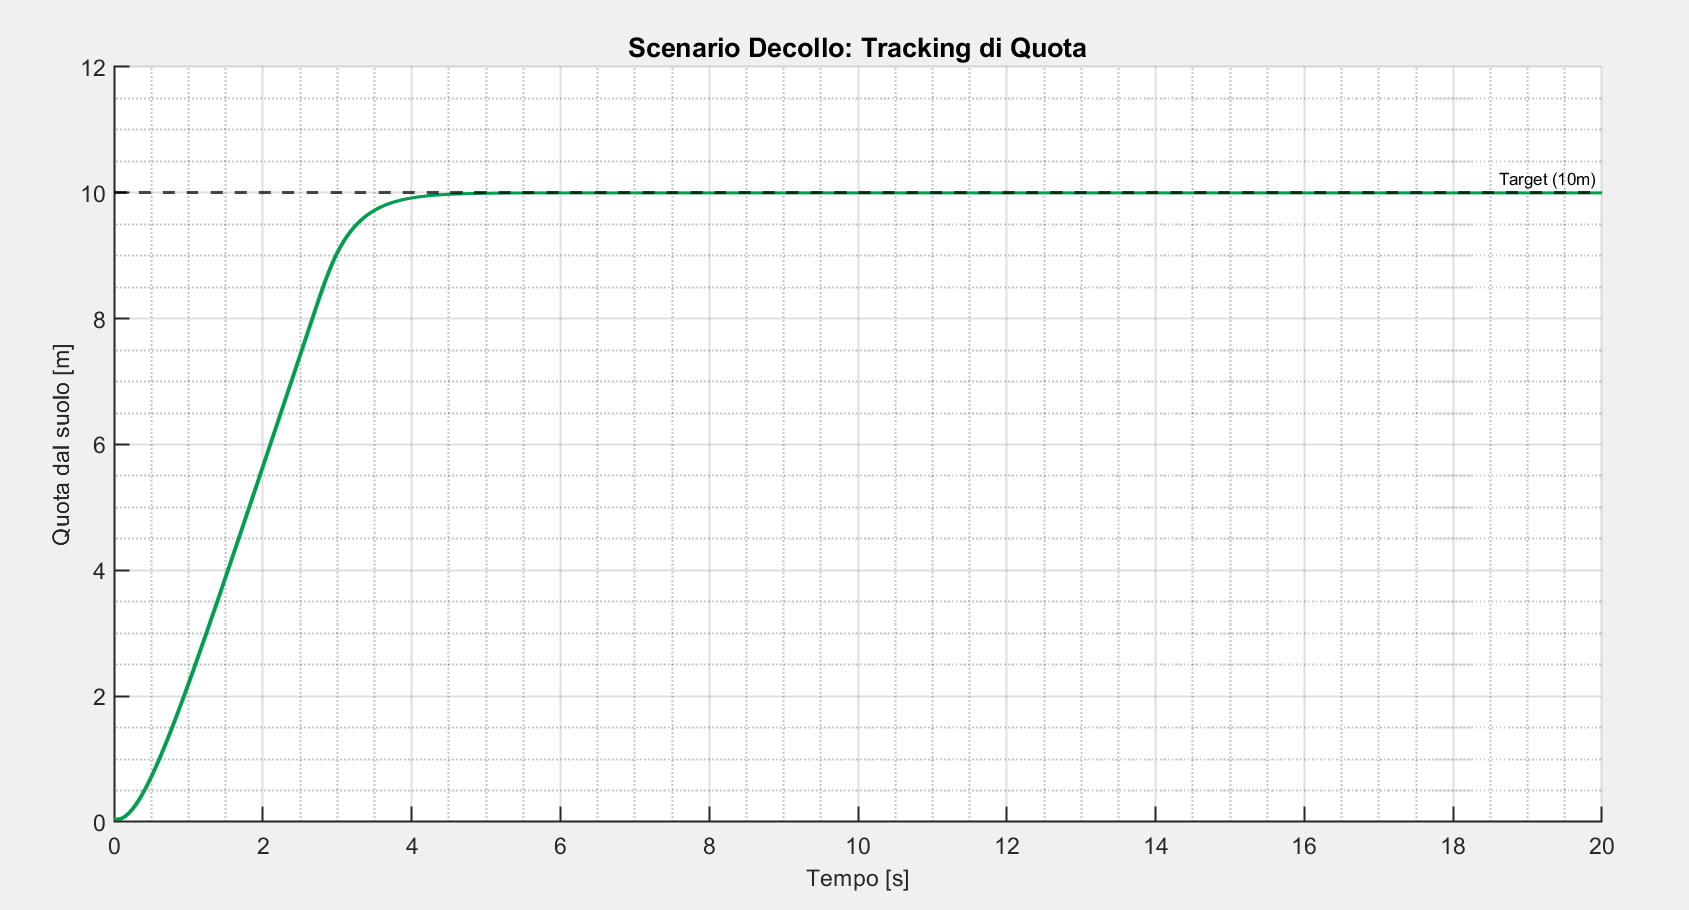
\includegraphics[width=\linewidth, height=5.5cm, keepaspectratio]{montecarlo/takeoff.png}
            \captionof{figure}{\footnotesize \textbf{Tracking Quota ($Z$):} Sovrapposizione di 100 simulazioni. Si nota la perfetta coincidenza delle traiettorie e la salita monotona da $0$ a $-10$m senza oscillazioni.}
        \end{column}
    \end{columns}
\end{frame}

% --- SLIDE 3: RECUPERO ---
\begin{frame}{Scenario 2: Recupero in Hovering (Recovery)}
    \textbf{Obiettivo:} Reiezione di disturbi severi su posizione e assetto.
    
    \vspace{0.1cm}
    % IMMAGINE: Inserisci qui 'Figure 1.1' (Posizione 3D o XYZ) oppure 'Figure 1.2' (Velocità)
    \centering
    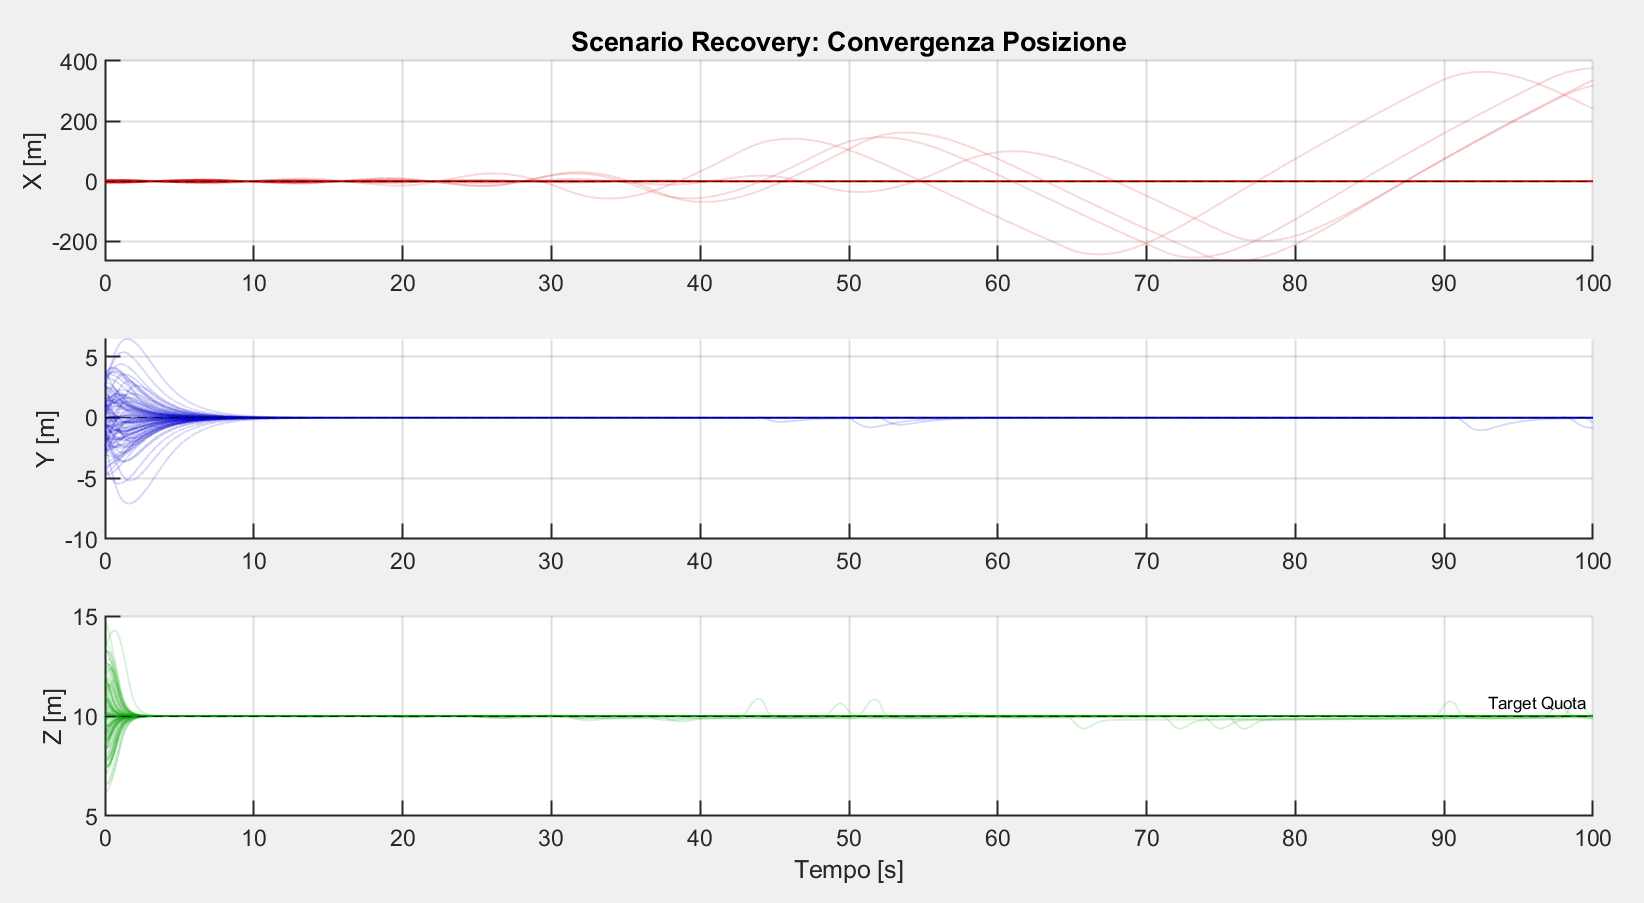
\includegraphics[width=0.9\linewidth, height=4.2cm, keepaspectratio]{montecarlo/recovery_V.png}
    \captionof{figure}{\footnotesize \textbf{Convergenza Posizione:} "Spaghetti plot" di 100 run. L'elevata dispersione iniziale (caos a $t=0$) viene completamente assorbita dal controllore, portando tutte le traiettorie a convergere nell'origine (Target).}
    
    \vspace{0.2cm}
    \begin{columns}[T]
        \begin{column}{0.33\textwidth}
            \centering
            \textbf{Success Rate}\\
            \textcolor{orange}{\Large 96\%}\\
            \tiny (4 outlier su 100)
        \end{column}
        \begin{column}{0.33\textwidth}
            \centering
            \textbf{RMSE Velocità}\\
            \Large 0.76 m/s\\
            \tiny Smorzamento efficace
        \end{column}
        \begin{column}{0.33\textwidth}
            \centering
            \textbf{Analisi Failure}\\
            \tiny I 4 casi falliti derivano da assetti iniziali estremi ($>60^\circ$) a bassa quota, fisicamente irrecuperabili.
        \end{column}
    \end{columns}
\end{frame}

% --- SLIDE 4: CROCIERA ---
\begin{frame}{Scenario 3: Volo di Crociera (Cruise)}
    \textbf{Obiettivo:} Verifica stabilità longitudinale a lungo termine ($t_{span}$ esteso).
    
    \vspace{0.3cm}
    \begin{columns}[c]
        \begin{column}{0.5\textwidth}
            \textbf{Performance Longitudinale:}
            \begin{itemize}
                \item \textbf{RMSE $V_x$:} \textcolor{green!60!black}{\textbf{3 mm/s}} (Drift nullo)
                \item \textbf{RMSE Quota:} \textcolor{green!60!black}{\textbf{2.9 cm}}
            \end{itemize}
            \vspace{0.2cm}
            \small
            \textit{L'assenza di deriva su $V_x$ conferma che la stima del drag e il feedforward sono corretti.}
        \end{column}
        
        \begin{column}{0.5\textwidth}
            \begin{alertblock}{Nota Dinamica Laterale}
                La posizione laterale ($Y$) è in \textbf{Open Loop}.
                Il drift osservato è fisiologico e non influenza la sicurezza del volo.
            \end{alertblock}
        \end{column}
    \end{columns}

    \vspace{0.2cm}
    \centering
    % IMMAGINE: Inserisci qui 'Figure 21.2' (Velocità Vx vs Tempo)
    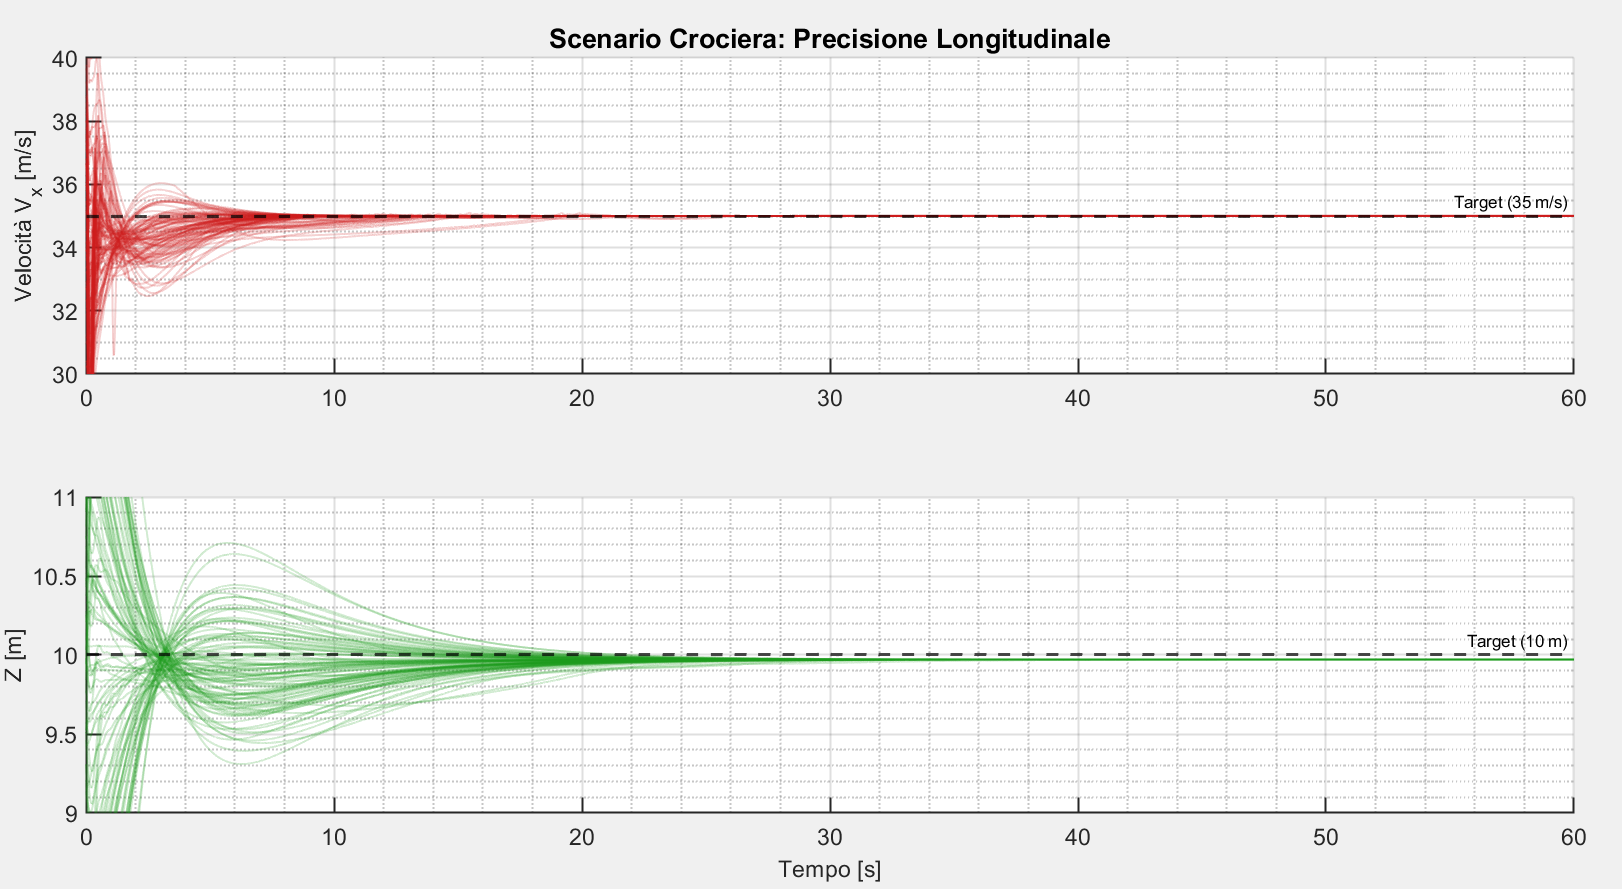
\includegraphics[width=0.85\linewidth, height=3.5cm, keepaspectratio]{montecarlo/cruise.png}
    \captionof{figure}{\footnotesize \textbf{Inseguimento $V_x$:} Le 100 linee si sovrappongono perfettamente sul target di $25$ m/s. Il "tubo" di errore è impercettibile, indicando altissima robustezza alle incertezze parametriche.}
\end{frame}

% --- SLIDE 5: SINTESI ---
\begin{frame}{Sintesi della Validazione ($N=300$)}
    \centering
    \Large
    Il sistema di controllo dimostra elevata affidabilità sull'intero inviluppo.
    
    \vspace{0.5cm}
    \normalsize
    \renewcommand{\arraystretch}{1.5}
    \begin{table}[]
        \centering
        \begin{tabular}{l c l}
            \toprule
            \textbf{Fase} & \textbf{Esito} & \textbf{Note} \\
            \midrule
            Decollo & \textcolor{green!60!black}{\textbf{OTTIMO}} & Transitorio nominale perfetto. \\
            Hovering & \textcolor{blue}{\textbf{ROBUSTO}} & 96\% Successo. Failure confinate a condizioni "Crash inevitabile". \\
            Crociera & \textcolor{green!60!black}{\textbf{OTTIMO}} & Stabilità asintotica confermata (No Drift). \\
            \bottomrule
        \end{tabular}
    \end{table}
\end{frame}


% ============================================================
% 5. CONCLUSIONI
% ============================================================
\section{Conclusioni}

\begin{frame}
    \vfill
    \centering
    {\Huge \textbf{Conclusioni}}
    \vfill
\end{frame}

\begin{frame}{Conclusioni e Sviluppi Futuri}
    \textbf{Risultati ottenuti:}
    \begin{itemize}
        \item Modellazione completa a 6-DOF per tricottero tilting-rotor.
        \item Sintesi del controllore per il volo verticale.
    \end{itemize}
    
    \vspace{0.8cm}
    \textbf{Sviluppi Futuri:}
    \begin{itemize}
        \item Sintesi controllore per il volo orizzontale.
        \item Analisi di stabilità.
    \end{itemize}
\end{frame}

% \begin{frame}
%     \centering
%     \Huge \textbf{Grazie per l'attenzione}
    
%     \vspace{1cm}
%     \Large Domande?
% \end{frame}

\end{document}
